\documentclass[10pt, aspectratio=169]{beamer}

% ============================================
% 테마 및 색상 설정
% ============================================
\usetheme{metropolis}
\usecolortheme{default}

% 색상 커스터마이징
\definecolor{myblue}{RGB}{0, 83, 159}
\definecolor{myorange}{RGB}{246, 168, 0}
\definecolor{mygray}{RGB}{100, 100, 100}

\setbeamercolor{frametitle}{bg=myblue, fg=white}
\setbeamercolor{title}{fg=myblue}
\setbeamercolor{structure}{fg=myblue}
\setbeamercolor{alerted text}{fg=myorange}

% ============================================
% 패키지
% ============================================
\usepackage{kotex}              % 한글 지원
\usepackage{amsmath, amssymb, amsthm}
\usepackage{graphicx}
\usepackage{booktabs}
\usepackage{hyperref}
\usepackage{tikz}
\usepackage{listings}

% 코드 스타일 설정
\lstset{
    basicstyle=\ttfamily\small,
    keywordstyle=\color{myblue}\bfseries,
    commentstyle=\color{mygray},
    stringstyle=\color{myorange},
    breaklines=true,
    frame=single,
    showstringspaces=false
}

% ============================================
% 문서 정보
% ============================================
\title{Algorithms for Reinforcement Learning}
\author{김응서}
\institute{SNU BI Lab (Seoul National University BioIntelligence Lab)}
\date{\today}

% ============================================
% 문서 시작
% ============================================
\begin{document}

% 타이틀 페이지
\begin{frame}
    \titlepage
\end{frame}

% 리뷰 대상 교재 정보
\begin{frame}{리뷰 대상 교재}
    \begin{block}{Algorithms for Reinforcement Learning}
        \textbf{저자:} Csaba Szepesvári
        
        \vspace{0.5em}
        \textbf{출판:} Morgan \& Claypool Publishers
        
        \vspace{0.5em}
        \textbf{시리즈:} Synthesis Lectures on Artificial Intelligence and Machine Learning
        
        \vspace{0.5em}
        \textbf{발행일:} June 9, 2009
    \end{block}
    
    \vspace{1em}
    \small{
    \textit{* 본 발표는 위 교재를 기반으로 하며, 김응서가 추가적으로 정리한 내용도 포함합니다.}
    }
\end{frame}

% 목차
\begin{frame}{교재 목차 (1/2)}
    \begin{enumerate}
        \item \textbf{Overview}
        
        \item \textbf{Markov Decision Processes}
        \begin{itemize}
            \item Preliminaries
            \item Markov Decision Processes
            \item Value functions
            \item Dynamic programming algorithms for solving MDPs
        \end{itemize}
        
        \item \textbf{Value Prediction Problems}
        \begin{itemize}
            \item Temporal difference learning in finite state spaces
            \begin{itemize}
                \item Tabular TD(0)
                \item Every-visit Monte-Carlo
                \item TD($\lambda$): Unifying Monte-Carlo and TD(0)
            \end{itemize}
            \item Algorithms for large state spaces
        \end{itemize}
    \end{enumerate}
\end{frame}

\begin{frame}{교재 목차 (2/2)}
    \begin{enumerate}
        \setcounter{enumi}{3}
        \item \textbf{Control}
        \begin{itemize}
            \item A catalog of learning problems
            \item Closed-loop interactive learning
            \item Direct methods (Q-learning)
            \item Actor-critic methods
        \end{itemize}
        
        \item \textbf{For Further Exploration}
        \begin{itemize}
            \item Further reading
            \item Applications
            \item Software
        \end{itemize}
        
        \vspace{0.5em}
        \textbf{Appendix:} The theory of discounted Markovian decision processes
    \end{enumerate}
\end{frame}

% ============================================
\section{Overview}
% ============================================

\begin{frame}{강화학습이란?}
    \begin{block}{Reinforcement Learning (RL)}
        Learning to control a system so as to \textbf{maximize} some numerical value which represents a \textbf{long-term objective};;
    \end{block}
    
    \vspace{0.5em}
    \begin{center}
        \includegraphics[width=0.4\textwidth]{images/figure-1.png}
    \end{center}
    
    \vspace{0.3em}
    \small{\textit{Agent $\leftrightarrow$ Environment: State, Action, Reward의 순환}}
\end{frame}

\begin{frame}{유명 교재별 강화학습 정의 (1/4)}
    \footnotesize
    \begin{tabular}{p{2.8cm}p{7.5cm}}
        \toprule
        \textbf{저자} & \textbf{정의} \\
        \midrule
        Sutton \& Barto & "Reinforcement learning problems involve learning \textbf{what to do—how to map situations to actions}—so as to \textbf{maximize a numerical reward signal}." \\
        & \textit{→ 상황$\rightarrow$행동을 학습해 보상(수치 신호) 최대화} \\
        \midrule
        Sutton \& Barto & "Reinforcement learning is a \textbf{computational approach} to understanding and automating \textbf{goal-directed learning} and \textbf{decision-making}." \\
        & \textit{→ 목표지향적 학습·의사결정을 이해/자동화하려는 계산적 접근} \\
        \bottomrule
    \end{tabular}
    
    \vspace{0.3em}
    \tiny{\textit{Source: Reinforcement Learning: An Introduction (2nd ed.)}}
\end{frame}

\begin{frame}{유명 교재별 강화학습 정의 (2/4)}
    \footnotesize
    \begin{tabular}{p{2.8cm}p{7.5cm}}
        \toprule
        \textbf{저자} & \textbf{정의} \\
        \midrule
        Kaelbling, Littman, Moore & "Reinforcement learning is the problem faced by \textbf{an agent that learns behavior} through \textbf{trial-and-error interactions} with a dynamic environment." \\
        & \textit{→ 동적 환경과 상호작용하며 시행착오로 행동을 학습} \\
        \midrule
        David Silver & "The agent's job is to \textbf{maximise cumulative reward}." \\
        & \textit{→ 에이전트의 목적은 누적 보상 최대화} \\
        \midrule
        David Silver & "The \textbf{environment is initially unknown} / The agent \textbf{interacts} with the environment / The agent \textbf{improves its policy}" \\
        & \textit{→ 환경이 미지인 상태에서 상호작용으로 정책을 개선} \\
        \bottomrule
    \end{tabular}
    
    \vspace{0.3em}
    \tiny{\textit{Sources: "Reinforcement Learning: A Survey" (JAIR); UCL RL Lecture 1}}
\end{frame}


\begin{frame}{유명 교재별 강화학습 정의 (3/4)}
    \footnotesize
    \begin{tabular}{p{2.8cm}p{7.5cm}}
        \toprule
        \textbf{저자} & \textbf{정의} \\
        \midrule
        Bertsekas & "Reinforcement learning, \textbf{approximate dynamic programming}, and \textbf{neuro-dynamic programming}." \\
        & \textit{→ RL을 (근사)동적계획/최적제어 큰 틀(ADP·NDP)로 규정} \\
        \midrule
        Bertsekas & "Our subject has benefited greatly from the \textbf{interplay of ideas from optimal control and from artificial intelligence}." \\
        & \textit{→ 최적제어와 AI의 접점/상호작용에서 발전} \\
        \midrule
        Andrew Ng & "Our goal in reinforcement learning is to \textbf{choose actions over time} so as to \textbf{maximize the expected value of the total payoff}." \\
        & \textit{→ 시간에 걸쳐 행동을 선택해 기대 보상 총합 최대화} \\
        \bottomrule
    \end{tabular}
    
    \vspace{0.3em}
    \tiny{\textit{Sources: Reinforcement Learning and Optimal Control (draft); Stanford CS229 Notes}}
\end{frame}

\begin{frame}{유명 교재별 강화학습 정의 (4/4)}
    \footnotesize
    \begin{tabular}{p{2.8cm}p{7.5cm}}
        \toprule
        \textbf{저자} & \textbf{정의} \\
        \midrule
        Szepesvári & "Reinforcement learning is a learning paradigm concerned with \textbf{learning to control a system} so as to maximize a numerical performance measure." \\
        & \textit{→ 시스템을 제어하는 정책을 학습해 장기 성능지표(수치) 최대화} \\
        \midrule
        Dayan \& Niv & "Animals learn to \textbf{choose actions to obtain rewards} and \textbf{avoid punishments}." \\
        & \textit{→ 동물이 보상 획득/벌 회피를 위해 행동 선택을 학습하는 틀} \\
        \midrule
        Mnih et al. & "The theory of reinforcement learning provides a \textbf{normative account} of how agents may \textbf{optimize their control} of an environment." \\
        & \textit{→ 에이전트가 환경 제어를 최적화하는 방법에 대한 규범적 이론} \\
        \bottomrule
    \end{tabular}
    
    \vspace{0.3em}
    \tiny{\textit{Sources: Algorithms for Reinforcement Learning; Dayan \& Niv (2008); Nature (2015) DQN}}
\end{frame}

\begin{frame}{주요 간단 용어 (1/3)}
    \begin{description}
        \item[\textbf{Environment (환경)}] Agent가 행동하는 공간
        
        \item[\textbf{State (상태) $s \in \mathcal{S}$}] 환경에서 agent가 있을 수 있는 여러 상태 중 하나
        
        \item[\textbf{Action (행동) $a \in \mathcal{A}$}] Agent가 한 상태에서 다른 상태로 전환하기 위해 선택할 수 있는 행동
        
        \item[\textbf{Reward (보상) $r \in \mathcal{R}$}] 행동을 취한 후 환경이 피드백으로 제공하는 보상
        
        \item[\textbf{Transition Probability (전이 확률) $P$}] 행동 후 어떤 상태에 도달할지 결정하는 확률
    \end{description}
\end{frame}

\begin{frame}{주요 간단 용어 (2/3)}
    \begin{description}
        \item[\textbf{Model}] 환경이 특정 행동에 어떻게 반응할지 정의 \\
        \small{보상 함수와 전이 확률을 포함}
        
        \vspace{0.3em}
        \item[\textbf{Policy (정책) $\pi(s)$}] 특정 상태에서 최적의 행동을 안내 \\
    \small{\alert{총 보상을 최대화}하는 것이 목표}
        
        \vspace{0.3em}
        \item[\textbf{Value Function $V(s)$}] 해당 상태에서 정책을 따를 때 받을 수 있는 미래 보상의 기댓값 예측 \\
        \small{상태가 얼마나 좋은지를 정량화}
    \end{description}
    
\end{frame}

\begin{frame}{주요 간단 용어 (3/3)}
    Agent와 environment의 상호작용은 시간에 따른 행동과 관찰된 보상의 \textbf{sequence}를 포함:
    
    \vspace{0.5em}
    시간 단계: $t = 1, 2, \ldots, T$
    
    \vspace{1em}
    \textbf{Notation:}
    \begin{itemize}
        \item $S_t$: 시간 $t$에서의 상태 (state)
        \item $A_t$: 시간 $t$에서의 행동 (action)
        \item $R_t$: 시간 $t$에서의 보상 (reward)
    \end{itemize}
    
    \vspace{1em}
    \begin{block}{Episode}
        하나의 완전한 상호작용 시퀀스 (또한 "\textbf{trial}" 또는 "\textbf{trajectory}"로 불림)
        
        \vspace{0.3em}
        Terminal state $S_T$에서 종료:
        $$S_1, A_1, R_2, S_2, A_2, \ldots, S_T$$
    \end{block}
\end{frame}

\begin{frame}{Model (1/3): Transition and Reward}
    \textbf{Model}은 환경의 descriptor로, 두 가지 주요 부분으로 구성:
    
    \vspace{0.5em}
    \begin{enumerate}
        \item \textbf{Transition Probability Function $P$}
        \item \textbf{Reward Function $R$}
    \end{enumerate}
    
    \vspace{1em}
    \begin{block}{Transition Step}
        상태 $s$에서 행동 $a$를 취해 다음 상태 $s'$에 도달하고 보상 $r$을 받음
        
        \vspace{0.3em}
        Tuple로 표현: $(s, a, s', r)$
    \end{block}
    
    \vspace{0.5em}
    \textbf{Transition Function:}
    $$P(s', r \mid s, a) = \mathbb{P}[S_{t+1} = s', R_{t+1} = r \mid S_t = s, A_t = a]$$
    
    \vspace{0.3em}
    \small{$\mathbb{P}$는 "probability"를 나타내는 기호}
\end{frame}

\begin{frame}{Model (2/3): State-Transition과 Reward Function}
    \textbf{State-Transition Function:}
    $$P_{ss'}^a = P(s' \mid s, a) = \mathbb{P}[S_{t+1} = s' \mid S_t = s, A_t = a] = \sum_{r \in \mathcal{R}} P(s', r \mid s, a)$$
    
    \vspace{1em}
    \textbf{Reward Function:}
    $$R(s, a) = \mathbb{E}[R_{t+1} \mid S_t = s, A_t = a] = \sum_{r\in\mathcal{R}} r \sum_{s' \in \mathcal{S}} P(s', r \mid s, a)$$
    
    \vspace{1em}
    \begin{itemize}
        \item Transition function은 행동 $a$ 후 상태 $s$에서 $s'$로 전환될 \textbf{확률}을 기록
        \item Reward function은 한 행동에 의해 발생하는 \textbf{다음 보상을 예측}
    \end{itemize}
\end{frame}

\begin{frame}{Model (3/3): Model-Based vs Model-Free RL}
    모델을 알고 있는지 여부에 따라 접근 방식이 달라짐:
    
    \vspace{1em}
    \begin{columns}[T]
        \begin{column}{0.48\textwidth}
            \begin{block}{Model-Based RL}
                \textbf{모델을 알고 있는 경우}
                \begin{itemize}
                    \item Dynamic Programming (DP) 사용 가능할 수도.
                \end{itemize}
            \end{block}
        \end{column}
        
        \begin{column}{0.48\textwidth}
            \begin{block}{Model-Free RL}
                \textbf{모델을 모르는 경우}
                \begin{itemize}
                    \item 그러니까 학습 시 모델에 의존적이지 않음.
                \end{itemize}
            \end{block}
        \end{column}
    \end{columns}
\end{frame}

\begin{frame}{Policy}
    \begin{block}{정의}
        Policy $\pi$는 agent의 \textbf{행동 함수(behavior function)}로, 상태 $s$에서 어떤 행동을 취할지 결정
    \end{block}
    
    \vspace{0.5em}
    상태 $s$에서 행동 $a$로의 매핑 (mapping from state to action)
    
    \vspace{1em}
    \textbf{두 가지 유형:}
    
    \begin{itemize}
        \item \textbf{Deterministic Policy (결정적 정책):}
        $$\pi(s) = a$$
        특정 상태에서 항상 같은 행동을 선택
        
        \vspace{0.5em}
        \item \textbf{Stochastic Policy (확률적 정책):}
        $$\pi(a \mid s) = \mathbb{P}_{\pi}[A = a \mid S = s]$$
        특정 상태에서 확률 분포에 따라 행동을 선택
    \end{itemize}
\end{frame}

\begin{frame}{Value Function (1/5)}
    \begin{block}{정의}
        Value function은 \textbf{상태 또는 행동이 얼마나 좋은지를} 미래 보상의 예측으로 측정
    \end{block}
    
    \vspace{0.5em}
    미래 보상(future reward)은 \textbf{return}이라고도 하며, 할인된 보상의 총합:
    
    \vspace{0.3em}
    $$G_t = R_{t+1} + \gamma R_{t+2} + \cdots = \sum_{k=0}^{\infty} \gamma^k R_{t+k+1}$$
    
    \vspace{0.5em}
    \textbf{Discounting factor: $\gamma \in [0, 1]$} \\
    \vspace{0.5em}
\end{frame}

\begin{frame}{Value Function (2/5): State-Value Function}
    \textbf{State-value function} $V_{\pi}(s)$: 시간 $t$에 상태 $s$에 있을 때의 기댓값 return
    
    $$V_{\pi}(s) = \mathbb{E}_{\pi}[G_t \mid S_t = s]$$
    
    \vspace{1em}
    \begin{itemize}
        \item 특정 정책 $\pi$를 따를 때 상태 $s$에서 기대되는 미래 보상의 총량
        \item "이 상태가 얼마나 좋은가?"에 대한 답
    \end{itemize}
\end{frame}

\begin{frame}{Value Function (3/5): Action-Value Function (Q-Value)}
    \textbf{Action-value function} $Q_{\pi}(s, a)$: 상태 $s$에서 행동 $a$를 취한 후의 기댓값 return
    
    $$Q_{\pi}(s, a) = \mathbb{E}_{\pi}[G_t \mid S_t = s, A_t = a]$$
    
    \vspace{0.5em}
    \begin{itemize}
        \item "Q-value"라고도 불림 (Q는 "Quality"를 의미)
        \item 특정 상태-행동 쌍의 가치를 평가
    \end{itemize}
    
    \vspace{1em}
    \textbf{State-value와의 관계:}
    
    정책 $\pi$를 따를 때, Q-value와 가능한 행동들의 확률 분포를 이용해 state-value 복원:
    
    $$V_{\pi}(s) = \sum_{a \in \mathcal{A}} Q_{\pi}(s, a) \pi(a \mid s)$$
\end{frame}

\begin{frame}{Value Function (4/5): Advantage Function}
    \textbf{Advantage function} $A_{\pi}(s, a)$: action-value와 state-value의 차이
    
    $$A_{\pi}(s, a) = Q_{\pi}(s, a) - V_{\pi}(s)$$
    
    \vspace{1em}
    \begin{itemize}
        \item "A-value"라고도 불림
        \item 특정 행동이 평균적인 행동보다 얼마나 더 좋은지를 나타냄
        \item $A_{\pi}(s, a) > 0$: 행동 $a$가 평균보다 좋음
        \item $A_{\pi}(s, a) < 0$: 행동 $a$가 평균보다 나쁨
        \item $A_{\pi}(s, a) = 0$: 행동 $a$가 평균 수준
    \end{itemize}
\end{frame}

\begin{frame}{Value Function (5/5): Optimal Value and Policy}
    \textbf{Optimal value function}은 최대 return을 생성:
    $$V_*(s) = \max_{\pi} V_{\pi}(s), \quad Q_*(s, a) = \max_{\pi} Q_{\pi}(s, a)$$
    
    \vspace{0.2em}
    \textbf{Optimal policy} $\pi_*$는 optimal value functions를 달성:
    $$\pi_* = \arg\max_{\pi} V_{\pi}(s), \quad \pi_* = \arg\max_{\pi} Q_{\pi}(s, a)$$
    
    \vspace{0.2em}
    당연히, 다음이 성립:
    $$V_{\pi_*}(s) = V_*(s) \quad \text{and} \quad Q_{\pi_*}(s, a) = Q_*(s, a)$$
    
    \vspace{0.2em}
    \begin{itemize}
        \item 모든 상태에서 최대 기댓값 return을 제공하는 정책이 optimal policy
        \item RL의 목표: optimal policy $\pi_*$를 찾는 것
    \end{itemize}
\end{frame}

% ============================================
\section{Markov Decision Processes: in an Easy way}
% ============================================

\begin{frame}{Markov Decision Processes (MDP) (1/2)}
    \textbf{거의 모든 RL 문제는 MDP로 표현 가능}
    
    \vspace{0.5em}
    MDP의 모든 상태는 "\textbf{Markov}" 속성을 가짐:
    
    \vspace{0.5em}
    \begin{block}{Markov Property}
        미래는 \textbf{현재 상태}에만 의존하며, 과거 이력에는 의존하지 않음
        
        $$\mathbb{P}[S_{t+1} \mid S_t] = \mathbb{P}[S_{t+1} \mid S_1, \ldots, S_t]$$
    \end{block}
    
    \vspace{0.5em}
    다시 말해, \textbf{미래와 과거는 현재 주어진 상황에서 조건부 독립}
    
    \vspace{0.5em}
    $\rightarrow$ 현재 상태가 미래를 결정하는 데 필요한 모든 통계를 포함
\end{frame}

\begin{frame}{Markov Decision Processes (MDP) (2/2)}
    \textbf{MDP는 5개의 요소로 구성:} $\mathcal{M} = \langle \mathcal{S}, \mathcal{A}, P, R, \gamma \rangle$
    
    \vspace{0.5em}
    \begin{itemize}
        \item $\mathcal{S}$ - 상태의 집합 (a set of states)
        \item $\mathcal{A}$ - 행동의 집합 (a set of actions)
        \item $P$ - 전이 확률 함수 (transition probability function)
        \item $R$ - 보상 함수 (reward function)
        \item $\gamma$ - 미래 보상에 대한 할인 계수 (discounting factor for future rewards)              
    \end{itemize}
\end{frame}

\begin{frame}{MDP Example: A Typical Work Day}
    \begin{center}
        \includegraphics[width=0.7\textwidth]{images/mdp_example.jpg}
    \end{center}
    \vspace{0.1em}
    \small{A fun example of Markov decision process: a typical work day.}
    \vspace{0.05em}
    \tiny{Image source: randomant.net/reinforcement-learning-concepts}
\end{frame}

\begin{frame}{Bellman Equations}
    \textbf{Bellman equations} decompose the value function into \textbf{immediate reward} and \textbf{discounted future values}:
    
    \vspace{0.5em}
    \textbf{State-Value Function:}
    \begin{align*}
        V(s) &= \mathbb{E}[G_t \mid S_t = s] \\
        &= \mathbb{E}[R_{t+1} + \gamma R_{t+2} + \gamma^2 R_{t+3} + \cdots \mid S_t = s] \\
        &= \mathbb{E}[R_{t+1} + \gamma(R_{t+2} + \gamma R_{t+3} + \cdots) \mid S_t = s] \\
        &= \mathbb{E}[R_{t+1} + \gamma G_{t+1} \mid S_t = s] \\
        &= \mathbb{E}[R_{t+1} + \gamma V(S_{t+1}) \mid S_t = s]
    \end{align*}
    
    \vspace{0.5em}
    \textbf{Action-Value Function (Q-value):}
    \begin{align*}
        Q(s, a) &= \mathbb{E}[R_{t+1} + \gamma V(S_{t+1}) \mid S_t = s, A_t = a] \\
        &= \mathbb{E}[R_{t+1} + \gamma \mathbb{E}_{a \sim \pi} Q(S_{t+1}, a) \mid S_t = s, A_t = a]
    \end{align*}
\end{frame}

\begin{frame}{Built-in Assumptions}
    \textbf{Core Idea:} The optimal value of a state is the best expected return achievable from that state onward.
    
    \vspace{0.3em}
    \begin{columns}[c]
        \begin{column}{0.48\textwidth}
            \centering
            $V^\pi(s) = E_\pi\left[\sum_{t=0}^{T} \gamma^t r_t \mid s_0 = s\right]$
        \end{column}
        
        \begin{column}{0.48\textwidth}
            \centering
            $V^*(s) = \max_a E_{s'} [r(s,a) + \gamma V^*(s')]$
        \end{column}
    \end{columns}
    
    \vspace{0.8em}
    \textbf{Built-in Assumptions:}
    \begin{itemize}
        \item \textbf{Markovian} - 미래는 현재 상태에만 의존 (과거 이력 무관)
        \item \textbf{Stationarity} - 환경의 동역학과 보상 함수가 시간에 따라 변하지 않음
        \item \textbf{Scalar rewards} - 보상은 단일 스칼라 값
        \item \textbf{Additivity of rewards} - 보상은 시간에 따라 가산적으로 누적
        \item \textbf{Estimation} - Value function을 근사 가능하다고 가정
        \item \textbf{Uniqueness} - 최적 value function이 존재
    \end{itemize}
    
    \vspace{0.5em}
    \small{\textit{Source: Joelle Pineau: Beyond Bellman's Legacy: Rethinking What we Value}}
\end{frame}

% ============================================
\section{Markov Decision Processes: in a Harder way}
% ============================================

\begin{frame}{Preliminaries: 표기}
    \textbf{Sets and Spaces:}
    \begin{itemize}
        \item $\mathbb{N}$ - Natural numbers: $\mathbb{N} = \{0, 1, 2, \ldots\}$
        \item $\mathbb{R}$ - Real numbers
        \item $v$ - Column vector, $v^{\top}$ - Row vector
    \end{itemize}
    
    \vspace{0.5em}
    \textbf{Inner Product and Norms:}
    \begin{itemize}
        \item Inner product: $\langle u, v \rangle = \sum_{i=1}^{d} u_i v_i$
        \item 2-norm: $\|u\|_2 = \sqrt{\langle u, u \rangle}$
        \item Max norm: $\|u\|_{\infty} = \max_{i=1,\ldots,d} |u_i|$
        \item Function norm: $\|f\|_{\infty} = \sup_{x \in X} |f(x)|$
    \end{itemize}
\end{frame}

\begin{frame}{Preliminaries: 주요 개념}
    \textbf{Lipschitz Mapping:}
    
    두 거리 공간 $(M_1, d_1)$, $(M_2, d_2)$ 사이의 매핑 $T$가 Lipschitz 상수 $L$을 가지면:
    $$d_2(T(a), T(b)) \leq L \cdot d_1(a, b), \quad \forall a, b \in M_1$$
    
    \begin{itemize}
        \item $L \leq 1$: \textbf{Non-expansion} (비확장)
        \item $L < 1$: \textbf{Contraction} (수축)
    \end{itemize}
    
    \vspace{1em}
    \textbf{Other Notations:}
    \begin{itemize}
        \item $I\{S\}$ - Indicator function: $S$가 참이면 1, 아니면 0
        \item $\frac{\partial}{\partial \theta} v$ - Partial derivative w.r.t. $\theta$ (row vector)
        \item $\nabla_{\theta} v$ - Gradient (column vector)
        \item $X \sim P$ - Random variable $X$ is drawn from distribution $P$
    \end{itemize}
\end{frame}

\begin{frame}[shrink=20]{Markov Decision Processes (MDP): Recap}
\small
\textbf{Concept:} A framework for modeling sequential decision-making problems where an agent observes states, selects actions, and probabilistically receives next states and rewards.
\vspace{0.15em}

\textbf{An MDP consists of 5 components:} $\mathcal{M} = \langle \mathcal{S}, \mathcal{A}, P, R, \gamma \rangle$
\begin{itemize}
    \item $\mathcal{S}$: set of states, \quad $\mathcal{A}$: set of actions
    \item $P$: transition probability function $P(s,a,s') = \Pr(S_{t+1}=s' \mid S_t=s, A_t=a)$
    \item $R$: reward function $R(s,a) = \mathbb{E}[R_{t+1}\mid S_t=s, A_t=a]$
    \item $\gamma \in [0,1]$: discount factor
\end{itemize}
\vspace{0.15em}

\textbf{Transition dynamics:}
\[
S_0 \sim \rho,\;
A_t \sim \pi(\cdot \mid S_t),\;
S_{t+1} \sim P(\cdot \mid S_t, A_t),\;
R_{t+1} \sim R(S_t, A_t)
\]
\vspace{0.15em}

\textbf{Objective:} Maximize expected discounted cumulative reward
\[
G = \sum_{t=0}^{\infty} \gamma^{t} R_{t+1},
\qquad
\pi^* \in \arg\max_{\pi}\; \mathbb{E}_{\pi}[G]
\]
\end{frame}

\begin{frame}{Value Functions: Motivation}
\textbf{Why value functions?}
\vspace{0.2em}

\textbf{Naive approach:} List all possible behaviors and identify optimal ones for each initial state
\begin{itemize}
    \item The number of deterministic policies: $|\Pi| = |\mathcal{A}|^{|\mathcal{S}|}$ \footnotemark
    \item Problem: \textbf{exponential complexity} in the number of states $\rightarrow$ computationally infeasible
\end{itemize}
\footnotetext[1]{\tiny \url{https://math.stackexchange.com/questions/4449548}}
\vspace{0.25em}

\textbf{Better approach:} Compute value functions
\begin{enumerate}
    \item First, compute the \textbf{optimal value function}
    \item Then, derive an optimal policy with relative ease
\end{enumerate}
\end{frame}

\begin{frame}{Stationary Policies (1/2)}
\textbf{Deterministic stationary policy:} A mapping $\pi: \mathcal{S} \to \mathcal{A}$
\[
A_t = \pi(S_t), \quad \forall t \geq 0
\]

\vspace{0.5em}
\textbf{Stochastic stationary policy:} Maps states to distributions over actions
\[
A_t \sim \pi(\cdot \mid S_t), \quad \forall t \geq 0
\]
where $\pi(a|s)$ denotes the probability of selecting action $a$ in state $s$.

\vspace{0.5em}
\textbf{Notation:} 
\begin{itemize}
    \item $\Pi_{\text{stat}}$ denotes the set of all stationary policies
    \item In what follows, "policy" means "stationary policy" unless stated otherwise
\end{itemize}
\end{frame}

\begin{frame}{Stationary Policies (2/2): Markov Reward Process}
\textbf{Markov Reward Process (MRP):} Induced by a stationary policy $\pi$ and MDP $\mathcal{M}$

\vspace{0.4em}
\textbf{Definition:} Determined by $(\mathcal{S}, P^\pi)$ where
\[
P^\pi(\cdot | s) = \sum_{a \in \mathcal{A}} \pi(a|s) P(\cdot | s, a)
\]

\vspace{0.5em}
\textbf{Key properties:}
\begin{itemize}
    \item The state process $(S_t; t \geq 0)$ becomes a time-homogeneous Markov chain
    \item Generates stochastic process $((S_t, R_{t+1}); t \geq 0)$
    \item Simplifies analysis by removing action selection decisions
\end{itemize}
\end{frame}

\begin{frame}{Value Functions (1/2): Policy Value Functions}
Fix a policy $\pi \in \Pi_{\text{stat}}$. Assume $\mathbb{P}(S_0 = s) > 0$ for all $s \in \mathcal{S}$.

\vspace{0.5em}
\textbf{State-value function} $V^\pi: \mathcal{S} \to \mathbb{R}$ underlying policy $\pi$:
\[
V^\pi(s) = \mathbb{E}\left[ \sum_{t=0}^{\infty} \gamma^t R_{t+1} \,\bigg|\, S_0 = s \right], \quad s \in \mathcal{S}
\]

\vspace{0.5em}
\textbf{Action-value function} $Q^\pi: \mathcal{S} \times \mathcal{A} \to \mathbb{R}$ underlying policy $\pi$:
\[
Q^\pi(s, a) = \mathbb{E}\left[ \sum_{t=0}^{\infty} \gamma^t R_{t+1} \,\bigg|\, S_0 = s, A_0 = a \right]
\]
where $(s,a) \in \mathcal{S} \times \mathcal{A}$.
\end{frame}

\begin{frame}{Value Functions (2/2): Optimal Value Functions}
\textbf{Optimal state-value function} $V_*: \mathcal{S} \to \mathbb{R}$:
\[
V_*(s) = \sup_{\pi \in \Pi_{\text{stat}}} V^\pi(s), \quad s \in \mathcal{S}
\]

\vspace{0.5em}
\textbf{Optimal action-value function} $Q_*: \mathcal{S} \times \mathcal{A} \to \mathbb{R}$:
\[
Q_*(s, a) = \sup_{\pi \in \Pi_{\text{stat}}} Q^\pi(s, a), \quad (s,a) \in \mathcal{S} \times \mathcal{A}
\]

\vspace{0.5em}
\textbf{Interpretation:}
\begin{itemize}
    \item $V_*(s)$: highest expected return achievable from state $s$
    \item $Q_*(s,a)$: highest expected return when starting from $s$ and taking action $a$ first
\end{itemize}
\end{frame}

\begin{frame}{Optimal Value Functions: Properties}
\textbf{Connection between} $V_*$ \textbf{and} $Q_*$:
\[
V_*(s) = \sup_{a \in \mathcal{A}} Q_*(s, a), \quad s \in \mathcal{S}
\]
\[
Q_*(s, a) = R(s, a) + \gamma \sum_{s' \in \mathcal{S}} P(s, a, s') V_*(s'), \quad (s,a) \in \mathcal{S} \times \mathcal{A}
\]

\vspace{0.6em}
\textbf{Optimal policy existence:} 
\begin{itemize}
    \item An optimal stationary policy always exists in the class of MDPs considered
    \item We have: $V_*(s) = \sup_{\pi \in \Pi_{\text{stat}}} V^\pi(s)$ for all $s \in \mathcal{S}$
\end{itemize}
\end{frame}

\begin{frame}{Optimal Policies and Greedy Actions}
\textbf{Characterization of optimal policies:} 

A policy $\pi \in \Pi_{\text{stat}}$ is optimal if and only if
\[
\sum_{a \in \mathcal{A}} \pi(a|s) Q_*(s, a) = V_*(s), \quad \forall s \in \mathcal{S}
\]

\vspace{0.6em}
\textbf{Greedy action:} An action $a$ is \emph{greedy} w.r.t. $Q$ in state $s$ if
\[
a \in \arg\max_{a' \in \mathcal{A}} Q(s, a')
\]

\vspace{0.6em}
\textbf{Key result:} A greedy policy w.r.t. $Q_*$ is optimal
\begin{itemize}
    \item Knowing $Q_*$ alone is sufficient for finding an optimal policy
    \item Knowing $V_*$, $R$, and $P$ also suffices to act optimally
\end{itemize}
\end{frame}

\begin{frame}{Bellman Equations for Policy Evaluation (1/2)}
\textbf{Goal:} Compute $V^\pi$ for a given policy $\pi$

\vspace{0.5em}
\textbf{Bellman equation for} $V^\pi$ (deterministic policy):
\[
V^\pi(s) = R(s, \pi(s)) + \gamma \sum_{s' \in \mathcal{S}} P(s, \pi(s), s') V^\pi(s'), \quad \forall s \in \mathcal{S}
\]

\vspace{0.5em}
\textbf{Bellman operator} $T^\pi: \mathbb{R}^\mathcal{S} \to \mathbb{R}^\mathcal{S}$:
\[
(T^\pi V)(s) = R(s, \pi(s)) + \gamma \sum_{s' \in \mathcal{S}} P(s, \pi(s), s') V(s')
\]

\vspace{0.5em}
Compact form: $T^\pi V^\pi = V^\pi$ (fixed-point equation)
\end{frame}

\begin{frame}{Bellman Equations for Policy Evaluation (2/2)}
\textbf{Properties of} $T^\pi$:
\begin{itemize}
    \item $T^\pi$ is an \textbf{affine linear} operator
    \item If $0 < \gamma < 1$, then $T^\pi$ is a \textbf{maximum-norm contraction}
    \item The fixed-point equation $T^\pi V = V$ has a \textbf{unique solution}
\end{itemize}

\vspace{0.6em}
\textbf{Finite state space:} 

For $|\mathcal{S}| = D$, we can write
\[
V^\pi = (I - \gamma P^\pi)^{-1} r^\pi
\]
where $r^\pi \in \mathbb{R}^D$ and $P^\pi \in \mathbb{R}^{D \times D}$ are appropriately defined.
\end{frame}

\begin{frame}{Bellman Optimality Equations (1/2)}
\textbf{Bellman optimality equation for} $V_*$:
\[
V_*(s) = \sup_{a \in \mathcal{A}} \left\{ R(s, a) + \gamma \sum_{s' \in \mathcal{S}} P(s, a, s') V_*(s') \right\}, \quad \forall s \in \mathcal{S}
\]

\vspace{0.5em}
\textbf{Bellman optimality operator} $T_*: \mathbb{R}^\mathcal{S} \to \mathbb{R}^\mathcal{S}$:
\[
(T_* V)(s) = \sup_{a \in \mathcal{A}} \left\{ R(s, a) + \gamma \sum_{s' \in \mathcal{S}} P(s, a, s') V(s') \right\}
\]

\vspace{0.5em}
Compact form: $T_* V_* = V_*$ (fixed-point equation)
\end{frame}

\begin{frame}{Bellman Optimality Equations (2/2)}
\textbf{Properties of} $T_*$:
\begin{itemize}
    \item $T_*$ is a \textbf{nonlinear} operator (due to $\sup$)
    \item If $0 < \gamma < 1$, then $T_*$ is a \textbf{maximum-norm contraction}
    \item The fixed-point equation $T_* V = V$ has a \textbf{unique solution}
\end{itemize}

\vspace{0.6em}
\textbf{Bellman optimality equation for} $Q_*$:
\[
Q_*(s, a) = R(s, a) + \gamma \sum_{s' \in \mathcal{S}} P(s, a, s') \sup_{a' \in \mathcal{A}} Q_*(s', a')
\]
for all $(s,a) \in \mathcal{S} \times \mathcal{A}$.
\end{frame}

\begin{frame}{Value Iteration (VI)}
\textbf{Key idea:} Instead of enumerating policies, directly update the \textbf{value function} $V$

\vspace{0.5em}
\textbf{Update rule:}
\[
V_{k+1}(s) = \max_{a \in \mathcal{A}} \left( R(s,a) + \gamma \sum_{s' \in \mathcal{S}} P(s,a,s') V_k(s') \right)
\]

\vspace{0.5em}
\textbf{Convergence property:}
\begin{itemize}
    \item With sufficient iterations: $V_k \to V^*$ (optimal value function)
    \item Guaranteed by contraction mapping theorem (when $0 < \gamma < 1$)
\end{itemize}

\vspace{0.5em}
\textbf{Extracting optimal policy:} After convergence, use greedy action selection:
\[
\pi^*(s) \in \arg\max_{a \in \mathcal{A}} \left( R(s,a) + \gamma \sum_{s' \in \mathcal{S}} P(s,a,s') V^*(s') \right)
\]
\end{frame}

\begin{frame}{Value Iteration: Convergence Rate}
\textbf{Geometric convergence:} By Banach's fixed-point theorem,

The sequence $V_{k+1} = T_* V_k$ converges to $V^*$ at a \textbf{geometric rate}:
\[
\|V_k - V^*\|_\infty \leq \gamma^k \|V_0 - V^*\|_\infty
\]

\vspace{0.5em}
\textbf{Q-value version:} VI can also be applied to action-value functions:
\[
Q_{k+1} = T_* Q_k, \quad k \geq 0
\]
which also converges to $Q^*$ at a geometric rate.

\vspace{0.5em}
\textbf{Approximate optimality guarantee:} For greedy policy $\pi$ w.r.t. $Q$:
\[
V^\pi(s) \geq V^*(s) - \frac{2}{1-\gamma} \|Q - Q^*\|_\infty, \quad \forall s \in \mathcal{S}
\]

This means if $Q_k \approx Q^*$, then a greedy policy w.r.t. $Q_k$ is near-optimal.
\end{frame}

\begin{frame}{VI: Iteration Complexity (1/2)}
\textbf{Question:} How many iterations to achieve $\varepsilon$-accuracy?

\vspace{0.5em}
\textbf{Contraction property:} $T_*$ is a $\gamma$-contraction in sup-norm:
\[
\|T_* U - T_* V\|_\infty \leq \gamma \|U - V\|_\infty
\]

{\small
여기서 $U, V: \mathcal{S} \to \mathbb{R}$는 임의의 value function 후보들이고, \\
$\|U - V\|_\infty = \max_{s \in \mathcal{S}} |U(s) - V(s)|$ (최대 차이). \\
즉, 임의의 두 value function에 $T_*$를 적용하면 그 최대 차이가 $\gamma$배 이하로 줄어든단 소리.
}

\vspace{0.5em}
\textbf{Error bound after $k$ iterations:}
\[
\|V_k - V^*\|_\infty \leq \gamma^k \|V_0 - V^*\|_\infty
\]

\vspace{0.5em}
This shows the error decreases by a factor of $\gamma$ at each iteration.
\end{frame}

\begin{frame}{VI: Iteration Complexity (2/2)}
\textbf{Iteration count for $\varepsilon$-accuracy:} To achieve $\|V_k - V^*\|_\infty \leq \varepsilon$:
\[
\gamma^k \|V_0 - V^*\|_\infty \leq \varepsilon
\quad \Rightarrow \quad
k \geq \frac{\log(\|V_0 - V^*\|_\infty/\varepsilon)}{-\log \gamma}
\]

\vspace{0.5em}
Since $-\log \gamma \approx 1 - \gamma$ when $\gamma \to 1$:
\[
K(\varepsilon) = O\left(\frac{\log(1/\varepsilon)}{1-\gamma}\right)
\]

\vspace{0.5em}
\textbf{Interpretation:}
\begin{itemize}
    \item \textbf{Logarithmic} in $1/\varepsilon$: Very fast convergence!
    \item \textbf{Linear} in $1/(1-\gamma)$: Slower when $\gamma$ is close to 1
    \item Standard result in RL/MDP literature
\end{itemize}
\end{frame}

\begin{frame}{VI: Total Computational Cost}
\textbf{Total cost} = (Cost per iteration) $\times$ (Number of iterations)

\vspace{0.5em}
\textbf{Cost per iteration:}
\begin{itemize}
    \item Dense transitions: $O(|\mathcal{S}|^2|\mathcal{A}|)$
    \item Sparse transitions (branching factor $d$): $O(|\mathcal{S}||\mathcal{A}|d)$
\end{itemize}

\vspace{0.5em}
\textbf{Number of iterations for $\varepsilon$-accuracy:} $K(\varepsilon) = O\left(\frac{\log(1/\varepsilon)}{1-\gamma}\right)$

\vspace{0.5em}
\textbf{Total computational complexity:}
\begin{itemize}
    \item \textbf{Dense:} $\widetilde{O}\left(\frac{|\mathcal{S}|^2|\mathcal{A}|}{1-\gamma}\right)$ to reach $\varepsilon$-accuracy
    \item \textbf{Sparse:} $\widetilde{O}\left(\frac{|\mathcal{S}||\mathcal{A}|d}{1-\gamma}\right)$ to reach $\varepsilon$-accuracy
\end{itemize}

\vspace{0.3em}
{\small (The $\widetilde{O}$ notation hides logarithmic factors in $1/\varepsilon$)}
\end{frame}

\begin{frame}{VI Complexity (1/2): Dense Transitions}
\textbf{Transition probability:} $P(s,a,s')=\Pr(S_{t+1}=s'\mid S_t=s, A_t=a)$

\vspace{0.5em}
\textbf{Dense transition:} For many $(s,a)$, \textbf{many} $s'$ have non-zero probability

\vspace{0.5em}
When computing the expectation:
\[
\sum_{s'\in\mathcal{S}} P(s,a,s')V(s')
\]
we must sum over nearly all $s' \in \mathcal{S}$ since $P(s,a,s') \neq 0$ for most $s'$.

\vspace{0.6em}
\textbf{Computational cost:}
\begin{itemize}
    \item Per $(s,a)$ pair: $O(|\mathcal{S}|)$ operations
    \item Total states: $|\mathcal{S}|$, total actions: $|\mathcal{A}|$
    \item \textbf{One VI iteration: $O(|\mathcal{S}|^2|\mathcal{A}|)$}
\end{itemize}
\end{frame}

\begin{frame}{VI Complexity (2/2): Sparse Transitions}
\textbf{Sparse transition:} For each $(s,a)$, reachable next states are \textbf{limited to a few}

\vspace{0.35em}
\textbf{Definition of} $d$: Number of non-zero transition probabilities
\[
d = \left|\{s' \in \mathcal{S} : P(s,a,s') > 0\}\right| \quad \text{where } d \ll |\mathcal{S}|
\]

\vspace{0.35em}
When computing the expectation:
\[
\sum_{s'\in\mathcal{S}} P(s,a,s')V(s')
\]
we only need to sum over $d$ terms (non-zero probabilities).

\vspace{0.35em}
\textbf{Computational cost:}
\begin{itemize}
    \item Per $(s,a)$ pair: $O(d)$ operations
    \item \textbf{One VI iteration: $O(|\mathcal{S}||\mathcal{A}|d)$}
    \item Much faster when $d \ll |\mathcal{S}|$
\end{itemize}
\end{frame}

\begin{frame}{Policy Iteration (PI)}
\textbf{Alternative approach:} Alternate between policy evaluation and policy improvement

\vspace{0.5em}
\textbf{Algorithm:} Start with arbitrary policy $\pi_0$. At iteration $k \geq 0$:

\vspace{0.3em}
\begin{enumerate}
    \item \textbf{Policy Evaluation:} Compute $Q^{\pi_k}$ (or $V^{\pi_k}$) by solving:
    \[
    Q^{\pi_k} = T^{\pi_k} Q^{\pi_k}
    \]
    
    \vspace{0.2em}
    \item \textbf{Policy Improvement:} Define greedy policy w.r.t. $Q^{\pi_k}$:
    \[
    \pi_{k+1}(s) \in \arg\max_{a \in \mathcal{A}} Q^{\pi_k}(s,a)
    \]
\end{enumerate}

\vspace{0.5em}
\textbf{Key property:} Each iteration is guaranteed to improve (or maintain) the policy:
\[
V^{\pi_{k+1}}(s) \geq V^{\pi_k}(s), \quad \forall s \in \mathcal{S}
\]
\end{frame}

\begin{frame}{Value Iteration vs. Policy Iteration}
\begin{tabular}{|p{0.33\textwidth}|p{0.27\textwidth}|p{0.27\textwidth}|}
\hline
\textbf{Aspect} & \textbf{Value Iteration} & \textbf{Policy Iteration} \\
\hline
\textbf{Update} & $V_{k+1} = T_* V_k$ & Solve $V^{\pi_k} = T^{\pi_k} V^{\pi_k}$ \\
\hline
\textbf{Cost per step} & Low: single sweep & High: solve linear system \\
\hline
\textbf{Convergence} & Geometric rate & Fewer iterations \\
\hline
\textbf{Policy quality} & Implicit (via greedy) & Explicit improvement \\
\hline
\end{tabular}

\vspace{0.6em}
\textbf{Trade-off:}
\begin{itemize}
    \item \textbf{VI:} Fast per iteration, but may need many iterations
    \item \textbf{PI:} Slow per iteration (policy evaluation), but converges in fewer iterations
    \item PI gives a policy not worse than VI after $k$ iterations (if started with same $V_0$)
\end{itemize}
\end{frame}
% ============================================
\section{A. The Theory of Discounted Markovian Decision Processes}
% ============================================
\section{A.1. Contractions and Banach’s fixed-point theorem}

\begin{frame}{Definition 1 (Norm)}
\textbf{정의:} 실수 위의 벡터 공간 $V$에 대해, 함수 $f : V \to \mathbb{R}_0^+$가 다음 조건들을 만족하면 $V$ 위의 \textbf{norm}이라고 한다:

\vspace{1em}
\begin{enumerate}
    \item 어떤 $v \in V$에 대해 $f(v) = 0$이면 $v = 0$이다;
    
    \vspace{0.5em}
    \item 임의의 $\lambda \in \mathbb{R}$, $v \in V$에 대해 $f(\lambda v) = |\lambda| f(v)$;
    
    \vspace{0.5em}
    \item 임의의 $v, u \in V$에 대해 $f(v + u) \leq f(v) + f(u)$.
\end{enumerate}

\vspace{1em}
여기서 $f$ 또는 Norm이 정의된 벡터 공간을 \textbf{normed vector space}라고 한다.

\vspace{1em}
\textbf{참고:} Norm은 각 벡터에 음이 아닌 실수를 할당하는 함수이다. 이 값을 벡터의 "길이(length)" 또는 "norm"이라고 부르며, 벡터 $v$의 norm을 $\|v\|$로 표기한다.
\end{frame}

\begin{frame}{Example: Norm의 예시 (1)}
벡터 공간 $V = (\mathbb{R}^d, +, \lambda \cdot)$ 위의 norm들:

\vspace{1em}
\textbf{1. $\ell_p$ norm:} $p \geq 1$에 대해,
\[
\|v\|_p = \left( \sum_{i=1}^{d} |v_i|^p \right)^{1/p}
\]
\small{$p=2$일 때 Euclidean distance, $p=1$일 때 Manhattan distance}

\vspace{1em}
\textbf{2. $\ell_\infty$ norm:}
\[
\|v\|_\infty = \max_{1 \leq i \leq d} |v_i|
\]
\small{최대 성분 값으로 정의되는 Chebyshev distance (또는 supremum norm)}

\small{쉽게는, 각 성분의 절댓값을 전부 보고, 그중에서 가장 큰 값 하나를 고른다는 소리}

\small{여기서 $d$는 벡터 공간의 차원(dimension)을 나타냄}
\end{frame}

\begin{frame}{Example: Norm의 예시 (2)}
\textbf{3. Weighted norms:}
\[
\|v\|_p = \begin{cases}
\left( \sum_{i=1}^{d} \frac{|v_i|^p}{w_i} \right)^{1/p}, & \text{if } 1 \leq p < \infty; \\[1em]
\max_{1 \leq i \leq d} \frac{|v_i|}{w_i}, & \text{if } p = \infty,
\end{cases}
\]

\small{여기서 $w_i > 0$. 각 차원에 서로 다른 가중치를 부여하여 중요도를 조절}

\vspace{1em}
\textbf{4. Matrix-weighted 2-norm:}
\[
\|v\|_{2,P} = \sqrt{v^T P v}
\]
여기서 $P$는 고정된 positive definite matrix이다. ($P$는 대칭행렬 + 모든 고유값이 양수)

\small{Positive definite matrix로 각 차원 간 상관관계를 반영한 거리}

\small{Matrix-weighted 2-norm은 행렬 $P$로 공간을 변형한 뒤, 그 변형된 공간에서 벡터의 길이를 재는 norm이다.}
\end{frame}

\begin{frame}{함수 공간에서의 Norm}
벡터 공간뿐만 아니라 함수 공간에서도 norm을 정의할 수 있다.

\vspace{1em}
\textbf{예시:} $V$가 정의역 $X$ 위에서 bounded인 함수들의 벡터 공간이면,
\[
\|f\|_\infty = \sup_{x \in X} |f(x)|
\]

\vspace{1em}
\textbf{참고:} 함수 $f$가 bounded인 것은 정확히 $\|f\|_\infty < +\infty$를 의미한다.
\end{frame}

\begin{frame}{Definition 2 (Convergence in norm)}
\textbf{정의:} $\mathcal{V} = (V, \|\cdot\|)$를 normed vector space라 하고, $v_n \in V$를 벡터들의 수열($n \in \mathbb{N}$)이라 하자.

\vspace{1em}
수열 $(v_n; n \geq 0)$이 벡터 $v$로 \textbf{노름 $\|\cdot\|$에서 수렴한다(converge to $v$ in the norm)}는 것은 다음을 의미한다:
\[
\lim_{n \to \infty} \|v_n - v\| = 0
\]

이를 $v_n \to_{\|\cdot\|} v$로 표기한다.

\vspace{1em}
\textbf{참고:} $d$-차원 벡터 공간에서 $v_n \to_{\|\cdot\|} v$는 모든 성분이 수렴하는 것, 즉 각 $1 \leq i \leq d$에 대해 $v_{n,i} \to v_i$가 성립하는 것과 같다. (단, $v_{n,i}$는 $v_n$의 $i$번째 성분)
\end{frame}

\begin{frame}{무한차원 벡터 공간에서의 수렴}
\textbf{주의:} 무한차원 벡터 공간에서는 pointwise convergence와 norm convergence가 다르다!

\vspace{1em}
\textbf{예시:} $X = [0, 1]$이고 $X$ 위의 bounded 함수 공간을 고려하자. 다음과 같이 정의하면:
\[
f_n(x) = \begin{cases}
1, & \text{if } x < 1/n; \\
0, & \text{otherwise}.
\end{cases}
\]

그리고 $f$를 다음과 같이 정의하자:
\[
f(x) = \begin{cases}
1, & \text{if } x = 0; \\
0, & \text{if } x \neq 0.
\end{cases}
\]
\end{frame}

\begin{frame}{Pointwise vs Norm Convergence}
앞의 예시에서:

\vspace{1em}
\textbf{Pointwise convergence:} 각 $x$에 대해 $f_n(x) \to f(x)$
\begin{itemize}
    \item 즉, $f_n$은 $f$로 pointwise하게 수렴한다
\end{itemize}

\vspace{1em}
\textbf{그러나, Norm convergence는 성립하지 않는다:}
\[
\|f_n - f\|_\infty = 1 \not\to 0
\]

\vspace{1em}
$\Rightarrow$ 무한차원 공간에서는 pointwise convergence가 norm convergence를 함의하지 않는다!
\end{frame}

\begin{frame}{추가 예시: 박스 이동}
\textbf{함수 정의:}
\[
f_n(x) = \begin{cases}
1, & \text{if } n \leq x \leq n+1; \\
0, & \text{otherwise}.
\end{cases}
\]

\vspace{0.5em}
\small{높이 1짜리 박스가 오른쪽으로 계속 이동}

\vspace{1em}
\textbf{왜 pointwise 수렴?}
\begin{itemize}
    \item $x$를 하나 고정하면, 어느 순간부터 박스가 $x$를 지나쳐 감
    \item 이후로는 계속 0: $f_n(x) \to 0$
    \item 모든 $x$에서 0으로 감
\end{itemize}

\vspace{0.5em}
\textbf{Pointwise convergence to 0}
\end{frame}

\begin{frame}{박스 이동: Norm Convergence는?}
앞의 예시에서:

\vspace{1em}
\textbf{Norm convergence는 성립하지 않는다:}
\[
\|f_n - 0\|_\infty = \|f_n\|_\infty = \sup_{x} |f_n(x)| = 1 \not\to 0
\]

\vspace{1em}
\textbf{왜?}
\begin{itemize}
    \item 각 $n$마다 함수 $f_n$은 어딘가($[n, n+1]$ 구간)에서 여전히 1의 값을 가짐
    \item Supremum norm은 함수가 가질 수 있는 최댓값을 측정
    \item 박스가 오른쪽으로 계속 이동해도, 높이는 항상 1로 유지됨
\end{itemize}

\vspace{0.5em}
\textbf{Norm convergence 실패}
\end{frame}

\begin{frame}{Cauchy Sequence}
실수 수열 $(a_n; n \geq 0)$의 경우, 극한값을 모르더라도 수렴성을 검증할 수 있다.

\vspace{1em}
\textbf{Cauchy sequence:} 다음을 만족하는 수열
\[
\lim_{n \to \infty} \sup_{m \geq n} |a_n - a_m| = 0
\]

("진동이 사라지는 수열"이라는 이름이 더 직관적일 수 있다)

\vspace{1em}
\textbf{실수의 중요한 성질:} 모든 실수의 Cauchy sequence는 극한을 가진다.

\vspace{1em}
Cauchy sequence 개념은 normed vector space로 자연스럽게 확장된다.
\end{frame}

\begin{frame}{Definition 3 (Cauchy sequence)}
\textbf{정의:} $(v_n; n \geq 0)$을 normed vector space $\mathcal{V} = (V, \|\cdot\|)$의 벡터들의 수열이라 하자.

\vspace{1em}
$v_n$이 \textbf{Cauchy sequence}라는 것은 다음을 의미한다:
\[
\lim_{n \to \infty} \sup_{m \geq n} \|v_n - v_m\| = 0
\]

\vspace{2em}
\textbf{중요한 사실:} 모든 Cauchy sequence가 수렴하는 normed vector space는 특별하다!

\vspace{1em}
일부 Cauchy sequence가 극한을 가지지 않는 normed vector space의 예시도 존재한다.
\end{frame}

\begin{frame}{Definition 4 (Completeness)}
\textbf{정의:} Normed vector space $\mathcal{V}$가 \textbf{complete}라는 것은 다음을 의미한다:

\vspace{1em}
\begin{center}
Every Cauchy sequence in $\mathcal{V}$ converges with respect to the norm of the vector space.
\end{center}

\vspace{2em}
\textbf{의미:}
\begin{itemize}
    \item Completeness는 "빈 곳이 없다"는 느낌(?)
    \item 해석학과 최적화 이론에서 매우 중요한 성질
\end{itemize}
\end{frame}

\begin{frame}{Definition 5 (Banach space)}
\textbf{정의:} Complete normed vector space를 \textbf{Banach space}라고 한다.

\vspace{2em}
\textbf{Banach space의 예시:}
\begin{itemize}
    \item $(\mathbb{R}^d, \|\cdot\|_p)$ (모든 $p \geq 1$에 대해)
    \item Bounded function space $(B(X), \|\cdot\|_\infty)$
    \item $L^p$ spaces (이건 뭔지 모르겠네.)
\end{itemize}
\end{frame}

\begin{frame}{Definition 6 (Lipschitz, Contraction)}
\textbf{정의:} $\mathcal{V} = (V, \|\cdot\|)$를 normed vector space라 하자. Mapping $T : V \to V$에 대해:

\vspace{1em}
\textbf{1. L-Lipschitz:} 임의의 $u, v \in V$에 대해
\[
\|Tu - Tv\| \leq L\|u - v\|
\]
\small{두 점 사이의 거리를 최대 $L$배까지만 변화시킴}

\vspace{0.5em}
\textbf{2. Non-expansion:} $L \leq 1$인 Lipschitz mapping
\small{거리를 늘리지 않음 (유지하거나 줄임)}

\vspace{0.5em}
\textbf{3. Contraction:} $L < 1$인 Lipschitz mapping
\small{거리를 반드시 줄임! 이때 $L$을 \textbf{contraction factor}라 하고, $T$를 $L$-contraction이라 함}
\end{frame}

\begin{frame}{Lipschitz Mapping의 연속성}
\textbf{중요한 성질:} $T$가 Lipschitz이면 연속(continuous)이다.

\vspace{1em}
즉, $v_n \to_{\|\cdot\|} v$이면 $Tv_n \to_{\|\cdot\|} Tv$도 성립한다.

\vspace{2em}
\textbf{증명:}
\[
\|Tv_n - Tv\| \leq L\|v_n - v\| \to 0 \quad \text{as } n \to \infty
\]

\vspace{1em}
\small{입력이 가까우면 출력도 가까워진다는 의미}
\end{frame}

\begin{frame}{Definition 7 (Fixed Point)}
\textbf{정의:} $T : V \to V$를 어떤 mapping이라 하자.

\vspace{1em}
벡터 $v \in V$가 $T$의 \textbf{fixed point}라는 것은 다음을 의미한다:
\[
Tv = v
\]

\vspace{2em}
\textbf{의미:}
\begin{itemize}
    \item Fixed point는 mapping $T$를 적용해도 변하지 않는 점
    \item 일종의 "평형점" 또는 "불동점"
    \item RL에서는 optimal value function이 Bellman operator의 fixed point가 됨
\end{itemize}
\end{frame}

\begin{frame}{Theorem 1 (Banach's Fixed-Point Theorem)}
\textbf{정리:} $\mathcal{V}$를 Banach space라 하고, $T : V \to V$를 contraction mapping이라 하자.

\vspace{1em}
그러면:
\begin{enumerate}
    \item $T$는 \textbf{유일한(unique)} fixed point를 가진다
    
    \vspace{0.5em}
    \item 임의의 $v_0 \in V$에 대해, $v_{n+1} = Tv_n$으로 정의하면
    \[
    v_n \to_{\|\cdot\|} v^*
    \]
    여기서 $v^*$는 $T$의 유일한 fixed point
    
    \vspace{0.5em}
    \item 수렴은 \textbf{기하급수적(geometric)}이다:
    \[
    \|v_n - v^*\| \leq \gamma^n \|v_0 - v^*\|
    \]
\end{enumerate}

\vspace{0.5em}
\small{\textbf{의미:} Contraction을 반복 적용하면 항상 유일한 fixed point로 빠르게 수렴!}
\end{frame}

\begin{frame}{증명 개요}
\textbf{증명 전략:} $T$를 $\gamma$-contraction이라 하자 ($\gamma < 1$).

\vspace{0.5em}
\textbf{Step 1:} 수열 $(v_n)$이 수렴함을 보이기
\begin{itemize}
    \item $(v_n)$이 Cauchy sequence임을 보임
    \item Banach space는 complete이므로 수렴
\end{itemize}

\vspace{0.5em}
\textbf{Step 2:} 극한 $v^*$가 fixed point임을 보이기
\begin{itemize}
    \item $v_{n+1} = Tv_n$의 양변에 극한을 취함
\end{itemize}

\vspace{0.5em}
\textbf{Step 3:} Fixed point의 uniqueness 증명
\begin{itemize}
    \item 두 개의 fixed point가 있다고 가정하면 모순
\end{itemize}

\vspace{0.5em}
\textbf{Step 4:} Geometric convergence 증명
\end{frame}

\begin{frame}{증명 Part 1: Cauchy Sequence}
\textbf{목표:} $(v_n)$이 Cauchy sequence임을 보이기

\vspace{0.3em}
임의의 $k \geq 0$에 대해:
\begin{align*}
\|v_{n+k} - v_n\| &= \|Tv_{n-1+k} - Tv_{n-1}\| \\
&\leq \gamma \|v_{n-1+k} - v_{n-1}\| \\
&= \gamma \|Tv_{n-2+k} - Tv_{n-2}\| \\
&\leq \gamma^2 \|v_{n-2+k} - v_{n-2}\| \\
&\vdots \\
&\leq \gamma^n \|v_k - v_0\|
\end{align*}

\vspace{0.3em}
이제 $\|v_k - v_0\|$을 bound해야 함...
\end{frame}

\begin{frame}{증명 Part 2: Cauchy Sequence (계속)}
삼각부등식을 이용하면:
\[
\|v_k - v_0\| \leq \|v_k - v_{k-1}\| + \|v_{k-1} - v_{k-2}\| + \cdots + \|v_1 - v_0\|
\]

\vspace{0.3em}
각 항에 대해: $\|v_i - v_{i-1}\| \leq \gamma^{i-1} \|v_1 - v_0\|$

\vspace{0.3em}
따라서:
\begin{align*}
\|v_k - v_0\| &\leq (\gamma^{k-1} + \gamma^{k-2} + \cdots + 1) \|v_1 - v_0\| \\
&\leq \frac{1}{1-\gamma} \|v_1 - v_0\|
\end{align*}

\vspace{0.3em}
결론:
\[
\|v_{n+k} - v_n\| \leq \gamma^n \cdot \frac{1}{1-\gamma} \|v_1 - v_0\| \to 0 \text{ as } n \to \infty
\]

$(v_n)$은 Cauchy sequence! Banach space이므로 수렴. 극한을 $v^*$라 하자.
\end{frame}

\begin{frame}{증명 Part 3: Fixed Point \& Uniqueness}
\textbf{$v^*$가 fixed point임:}

$v_{n+1} = Tv_n$의 양변에 극한을 취하면:
\begin{itemize}
    \item 좌변: $v_{n+1} \to_{\|\cdot\|} v^*$
    \item 우변: $Tv_n \to_{\|\cdot\|} Tv^*$ (contraction은 연속)
\end{itemize}
따라서 $v^* = Tv^*$ ✓

\vspace{1em}
\textbf{Uniqueness:} $v, v'$가 모두 fixed point라 가정하면:
\begin{align*}
\|v - v'\| &= \|Tv - Tv'\| \\
&\leq \gamma \|v - v'\|
\end{align*}

$(1-\gamma)\|v - v'\| \leq 0$이고 $\gamma < 1$이므로 $\|v - v'\| = 0$

따라서 $v = v'$ ✓
\end{frame}

\begin{frame}{증명 Part 4: Geometric Convergence}
\textbf{목표:} $\|v_n - v^*\| \leq \gamma^n \|v_0 - v^*\|$를 보이기

\begin{align*}
\|v_n - v^*\| &= \|Tv_{n-1} - Tv^*\| \quad (\because v^* = Tv^*) \\
&\leq \gamma \|v_{n-1} - v^*\| \\
&= \gamma \|Tv_{n-2} - Tv^*\| \\
&\leq \gamma^2 \|v_{n-2} - v^*\| \\
&\vdots \\
&\leq \gamma^n \|v_0 - v^*\|
\end{align*}

\vspace{0.3em}
\textbf{결론:} $\gamma < 1$이므로 $\gamma^n \to 0$ exponentially fast!

오차가 기하급수적으로 감소 $\Rightarrow$ 매우 빠른 수렴
\end{frame}

\begin{frame}{Banach Fixed-Point Theorem의 의의}
이 정리는 세 가지를 모두 보장한다:

\vspace{1em}
\begin{enumerate}
    \item \textbf{Existence:} Fixed point가 존재한다
    
    \vspace{0.5em}
    \item \textbf{Uniqueness:} Fixed point가 유일하다
    
    \vspace{0.5em}
    \item \textbf{계산 방법 (Computation):} 임의의 점에서 시작해서 $v_{n+1} = Tv_n$을 반복하면 fixed point로 수렴한다
\end{enumerate}

\vspace{1em}
\textbf{RL에서의 중요성:}
\begin{itemize}
    \item Bellman operator가 contraction임을 보이면
    \item Value iteration, Policy iteration 등의 알고리즘이 수렴함을 보장
    \item Optimal value function의 existence와 uniqueness 보장
\end{itemize}
\end{frame}

\section{A.2. Application to MDPs}

\begin{frame}{Optimal Value Function 정의}
이 섹션에서는 $V^*$를 다음과 같이 정의한다:
\[
V^*(s) = \sup_{\pi \in \Pi_{\text{stat}}} V^\pi(s), \quad s \in S
\]

\vspace{1em}
\textbf{의미:}
\begin{itemize}
    \item $V^*(s)$는 stationary policy를 선택하여 달성할 수 있는 값의 상한
\end{itemize}
\end{frame}

\begin{frame}{Bounded Function Space $B(S)$}
\textbf{정의:} $B(S)$를 정의역이 $S$인 bounded 함수들의 공간이라 하자:
\[
B(S) = \{ V : S \to \mathbb{R} : \|V\|_\infty < +\infty \}
\]

\vspace{0.5em}
\small{(강화학습 문맥에서는 $V$를 value function으로 봐도 무방)}

\vspace{1em}
앞으로 $B(S)$를 norm $\|\cdot\|_\infty$가 주어진 normed vector space로 볼 것이다.

\vspace{1em}
\textbf{중요한 성질:} $(B(S), \|\cdot\|_\infty)$는 \textbf{complete}이다!

즉, $B(S)$는 Banach space이다.
\end{frame}

\begin{frame}{$B(S)$의 Completeness 증명}
\textbf{목표:} $(V_n; n \geq 0)$이 $B(S)$의 Cauchy sequence이면 수렴함을 보이기

\vspace{0.5em}
\textbf{증명:}
\begin{itemize}
    \item 임의의 $s \in S$에 대해, $(V_n(s); n \geq 0)$은 실수의 Cauchy sequence
    \item 실수는 complete이므로 $V_n(s) \to V(s)$로 수렴
    \item $V(s)$를 각 $s$의 극한으로 정의하면 $\|V_n - V\|_\infty \to 0$
\end{itemize}

\vspace{0.5em}
\textbf{직관:}
\begin{itemize}
    \item $(V_n)$이 norm $\|\cdot\|_\infty$에서 Cauchy sequence이므로
    \item $V_n(s)$가 $V(s)$로 수렴하는 속도가 $s$에 무관
    \item 따라서 uniform convergence 보장
\end{itemize}
\end{frame}

\begin{frame}{Bellman Operator $T^\pi$의 Recap}
임의의 stationary policy $\pi$에 대해, Bellman operator $T^\pi : B(S) \to B(S)$를 다음과 같이 정의:
\[
(T^\pi V)(s) = r(s, \pi(s)) + \gamma \sum_{s' \in S} P(s, \pi(s), s') V(s'), \quad s \in S
\]

\vspace{1em}
\textbf{Well-definedness:} $U \in B(S)$이면 $T^\pi U \in B(S)$도 성립

\vspace{1em}
\textbf{핵심 성질:}
\begin{enumerate}
    \item $V^\pi$는 $T^\pi$의 fixed point
    \item $T^\pi$는 $\gamma$-contraction
\end{enumerate}
\end{frame}

\begin{frame}{$V^\pi$는 $T^\pi$의 Fixed Point}
식 (7)로 정의된 $V^\pi$는 $T^\pi$의 fixed point이다:

\vspace{0.5em}
\begin{align*}
V^\pi(s) &= \mathbb{E}[R_1 | S_0 = s] + \gamma \sum_{s' \in S} P(s, \pi(s), s') \mathbb{E}\left[ \sum_{t=0}^\infty \gamma^t R_{t+2} \,\Big|\, S_1 = s' \right] \\
&= T^\pi V^\pi(s)
\end{align*}

\vspace{1em}
\textbf{의미:}
\begin{itemize}
    \item Immediate reward + Discounted future value
    \item Bellman equation의 해
\end{itemize}
\end{frame}

\begin{frame}{$T^\pi$는 Contraction}
\textbf{정리:} $T^\pi$는 $\gamma$-contraction이다.

\vspace{0.5em}
\textbf{증명:}
\begin{align*}
\|T^\pi U - T^\pi V\|_\infty &= \gamma \sup_{s \in S} \left| \sum_{s' \in S} P(s, \pi(s), s') (U(s') - V(s')) \right| \\
&\leq \gamma \sup_{s \in S} \sum_{s' \in S} P(s, \pi(s), s') |U(s') - V(s')| \quad \text{\small (Triangle ineq.)} \\
&\leq \gamma \sup_{s \in S} \sum_{s' \in S} P(s, \pi(s), s') \|U - V\|_\infty \quad \text{\small (sup norm 정의)} \\
&= \gamma \|U - V\|_\infty \quad \text{\scriptsize ($\sum_{s'} P = 1$)}
\end{align*}
\end{frame}

\begin{frame}{$V^\pi$ 계산 방법}
Banach fixed-point theorem에 의해:

\vspace{1em}
임의의 $V_0 \in B(S)$에서 시작하여 수열을 구성:
\[
V_0, \quad T^\pi V_0, \quad (T^\pi)^2 V_0, \quad (T^\pi)^3 V_0, \quad \ldots
\]

\vspace{1em}
이 수열은 $V^\pi$로 \textbf{기하급수적 속도로 수렴}한다!

\vspace{1em}
\textbf{수렴 속도:}
\[
\|(T^\pi)^n V_0 - V^\pi\|_\infty \leq \gamma^n \|V_0 - V^\pi\|_\infty
\]

\vspace{0.5em}
$\Rightarrow$ Policy evaluation의 이론적 근거
\end{frame}

\begin{frame}{Bellman Optimality Operator $T^*$}
Bellman optimality operator $T^* : B(S) \to B(S)$를 다음과 같이 정의:
\[
(T^* V)(s) = \sup_{a \in A} \left\{ r(s, a) + \gamma \sum_{s' \in S} P(s, a, s') V(s') \right\}, \quad s \in S
\]

\vspace{1em}
$T^*$도 well-defined: $V \in B(S)$이면 $T^* V \in B(S)$

\vspace{1em}
\textbf{목표:} $T^*$도 $\gamma$-contraction임을 보이자!
\end{frame}

\begin{frame}{보조 부등식}
먼저 다음 부등식을 주목하자:
\[
\left| \sup_{a \in A} f(a) - \sup_{a \in A} g(a) \right| \leq \sup_{a \in A} |f(a) - g(a)|
\]

\vspace{1em}
\textbf{증명 :} case analysis로 보일 수 있음

\vspace{1em}
\textbf{직관:}
\begin{itemize}
    \item 두 supremum의 차이는
    \item 각 점에서의 차이의 supremum보다 클 수 없다
\end{itemize}

\vspace{1em}
이 부등식을 $T^*$의 contraction 증명에 사용할 것이다.
\end{frame}

\begin{frame}{$T^*$는 Contraction}
\textbf{정리:} $T^*$는 $\gamma$-contraction이다.

\vspace{0.3em}
\textbf{증명:}
\begin{align*}
\|T^* U - T^* V\|_\infty &\leq \gamma \sup_{(s,a) \in S \times A} \sum_{s' \in S} P(s, a, s') |U(s') - V(s')| \\
&\leq \gamma \sup_{(s,a) \in S \times A} \sum_{s' \in S} P(s, a, s') \|U - V\|_\infty \\
&= \gamma \|U - V\|_\infty
\end{align*}

마지막 등식: $\sum_{s' \in S} P(s, a, s') = 1$

\vspace{1em}
$\Rightarrow$ $T^*$도 유일한 fixed point를 가지며, 반복 적용으로 기하급수적 수렴!
\end{frame}

\begin{frame}{Theorem 2: Characterization of Optimal Policy}
\textbf{정리:} $V$를 $T^*$의 fixed point라 하고, policy $\pi$가 $V$에 대해 greedy라고 하자:
\[
T^\pi V = T^* V
\]
그러면 $V = V^*$이고, $\pi$는 optimal policy이다.

\vspace{1em}
\textbf{의미:}
\begin{itemize}
    \item $T^*$의 fixed point를 찾으면 그것이 곧 $V^*$
    \item 그 fixed point에 대해 greedy한 policy가 optimal policy
    \item Value iteration의 이론적 근거
\end{itemize}
\end{frame}

\begin{frame}{Theorem 2 증명 (1/2)}
\textbf{Step 1:} 임의의 stationary policy $\pi$에 대해 $V^\pi \leq V$임을 보이기

\vspace{0.5em}
$T^\pi \leq T^*$임에 주목 (임의의 $W \in B(S)$에 대해 $T^\pi W \leq T^* W$)

\vspace{0.5em}
따라서:
\[
V^\pi = T^\pi V^\pi \leq T^* V^\pi
\]

$T^*$가 monotone이므로 ($U \leq W \Rightarrow T^* U \leq T^* W$):
\[
T^* V^\pi \leq (T^*)^2 V^\pi
\]

부등식을 연쇄시키면:
\[
V^\pi \leq (T^*)^n V^\pi \quad \text{for all } n \geq 0
\]

$T^*$가 contraction이므로 우변은 $V$로 수렴. 따라서 $V^\pi \leq V$.

$\pi$가 임의였으므로: $V^* \leq V$
\end{frame}

\begin{frame}{Theorem 2 증명 (2/2)}
\textbf{Step 2:} $T^\pi V = T^* V$인 policy $\pi$를 선택

\vspace{0.5em}
$V$가 $T^*$의 fixed point이므로:
\[
T^\pi V = T^* V = V
\]

$T^\pi$는 유일한 fixed point $V^\pi$를 가지므로:
\[
V^\pi = V
\]

\vspace{1em}
\textbf{결론:}
\begin{itemize}
    \item $V^* \leq V = V^\pi \leq V^*$
    \item 따라서 $V = V^*$
    \item $\pi$는 optimal policy \qed
\end{itemize}
\end{frame}

\begin{frame}{Existence of Greedy Policy}
\textbf{주의:} Theorem 2에서 $V$에 대해 greedy한 policy가 존재해야 함

\vspace{1em}
\textbf{존재 조건:}
\begin{itemize}
    \item \textbf{Finite action space:} 항상 존재
    \item \textbf{Infinite action space:} 추가적인 연속성 가정 필요
\end{itemize}

\vspace{1em}
\textbf{Greedy policy:}
\[
\pi(s) \in \arg\max_{a \in A} \left\{ r(s, a) + \gamma \sum_{s' \in S} P(s, a, s') V(s') \right\}
\]
\end{frame}

\begin{frame}{Theorem 3 (Policy Improvement Theorem)}
\textbf{정리:} Stationary policy $\pi_0$를 선택하고, $\pi$가 $V^{\pi_0}$에 대해 greedy라 하자:
\[
T^\pi V^{\pi_0} = T^* V^{\pi_0}
\]
그러면 $V^\pi \geq V^{\pi_0}$ (즉, $\pi$는 $\pi_0$의 improvement)

\vspace{1em}
\textbf{특히:}
\begin{itemize}
    \item 어떤 state $s$에서 $T^* V^{\pi_0}(s) > V^{\pi_0}(s)$이면: $V^\pi(s) > V^{\pi_0}(s)$ (strict improvement)
    \item $T^* V^{\pi_0} = V^{\pi_0}$이면: $\pi_0$은 이미 optimal policy
\end{itemize}

\vspace{0.5em}
$\Rightarrow$ Policy iteration의 이론적 근거
\end{frame}

\begin{frame}{Theorem 3 증명}
\textbf{증명:}
\[
T^\pi V^{\pi_0} = T^* V^{\pi_0} \geq T^{\pi_0} V^{\pi_0} = V^{\pi_0}
\]

양변에 $T^\pi$를 적용:
\[
(T^\pi)^2 V^{\pi_0} \geq T^\pi V^{\pi_0} \geq V^{\pi_0}
\]

계속 반복하면:
\[
(T^\pi)^n V^{\pi_0} \geq V^{\pi_0} \quad \text{for all } n \geq 0
\]

양변의 극한을 취하면: $V^\pi \geq V^{\pi_0}$ \qed

\vspace{0.5em}
\textbf{Strict improvement:} $(T^\pi)^n V^{\pi_0}(s) \geq T^* V^{\pi_0}(s) > V^{\pi_0}(s)$

극한을 취하면: $V^\pi(s) > V^{\pi_0}(s)$
\end{frame}

\begin{frame}{Theorem 3 증명: 세 번째 부분}
\textbf{$T^* V^{\pi_0} = V^{\pi_0}$이면 $\pi_0$가 optimal:}

\vspace{0.5em}
$T^* V^{\pi_0} = V^{\pi_0}$이면 $V^{\pi_0}$는 $T^*$의 fixed point

\vspace{0.5em}
$T^*$는 contraction이므로 유일한 fixed point $V$를 가짐

\vspace{0.5em}
따라서 $V = V^{\pi_0}$

\vspace{0.5em}
또한 $V^{\pi_0} \leq V^* \leq V$이므로:
\[
V^{\pi_0} = V^* = V
\]

$\Rightarrow$ $\pi_0$는 optimal policy \qed
\end{frame}

\begin{frame}{Corollary 4: Termination of Policy Iteration}
\textbf{Corollary:} MDP가 finite이면:
\begin{enumerate}
    \item Policy iteration은 유한 단계에서 terminate
    \item Termination 시 optimal policy를 반환
\end{enumerate}

\vspace{0.5em}
또한: Stationary policy가 optimal $\Leftrightarrow$ 그 value function이 $T^*$의 fixed point

\vspace{1em}
\textbf{증명:}
\begin{itemize}
    \item Theorem 3에 의해 policy 수열은 strictly improving
    \item Finite MDP에서는 policy의 개수가 유한
    \item 따라서 반드시 terminate
    \item Termination 시 $T^* V^\pi = T^\pi V^\pi = V^\pi$ $\Rightarrow$ $\pi$는 optimal \qed
\end{itemize}
\end{frame}

\begin{frame}{Corollary 5: Optimality of Greedy Policy}
\textbf{Corollary:} $V$를 $T^*$의 유일한 fixed point라 하자.

\vspace{1em}
\textbf{Part 1:} $V$에 대해 greedy한 모든 policy는 optimal policy이다.

\vspace{1em}
\textbf{Part 2:} Optimal stationary policy $\pi^*$가 존재하면:
\begin{itemize}
    \item $V = V^*$
    \item $\pi^*$는 $V^*$에 대해 greedy
\end{itemize}

\vspace{1em}
\textbf{의미:} Optimal policy는 정확히 $V^*$에 대해 greedy한 policy들이다!
\end{frame}

\begin{frame}{Corollary 5 증명}
\textbf{Part 1:} Theorem 2에서 바로 따름

\vspace{1em}
\textbf{Part 2 증명:}

$\pi^*$가 optimal stationary policy라 가정. 따라서 $V^{\pi^*} = V^*$

\vspace{0.5em}
$V^{\pi^*} = T^{\pi^*} V^{\pi^*} \leq T^* V^{\pi^*}$

\vspace{0.5em}
Corollary 4의 두 번째 부분에 의해: $T^* V^{\pi^*} = V^{\pi^*}$

\vspace{0.5em}
따라서:
\[
V^{\pi^*} \leq V^* \leq V = V^{\pi^*}
\]

모두 같으며: $T^{\pi^*} V^* = T^* V^*$ \qed

\vspace{1em}
\textbf{핵심:} Optimal policy $\Leftrightarrow$ $V^*$에 대해 greedy
\end{frame}

% ============================================
\section{Value Prediction Problems}
% ============================================

\begin{frame}{What is Value Prediction?}
How do we estimate the \textbf{Value Function $V$} in an \textbf{MRP (Markov Reward Process)}?

\vspace{1em}
\textbf{Problem Setup:}
\begin{itemize}
    \item States evolve according to Markov dynamics
    \item Rewards are generated based on states
    \item Goal: Estimate the discounted sum of future rewards starting from state $s$
\end{itemize}

\vspace{1em}
\textbf{Value Function:}
\[
V(s) = \mathbb{E}[G \mid S_0 = s]
\]

where $G = R_1 + \gamma R_2 + \gamma^2 R_3 + \cdots$ (Return)
\end{frame}

\begin{frame}{Why "Value Prediction"?}
Many real-world problems take the form of "expected cumulative future outcomes":

\vspace{1em}
\begin{itemize}
    \item \textbf{Probability} of future events
    \begin{itemize}
        \item e.g., machine failure probability, customer churn probability
    \end{itemize}
    
    \vspace{0.5em}
    \item \textbf{Expected time} until an event occurs
    \begin{itemize}
        \item e.g., mean waiting time, mean time to failure
    \end{itemize}
    
    \vspace{0.5em}
    \item \textbf{Value Function} under a policy
    \begin{itemize}
        \item State value $V^\pi(s)$, Action value $Q^\pi(s,a)$
    \end{itemize}
\end{itemize}
\end{frame}

\begin{frame}{Monte-Carlo (MC) Methods}
\textbf{핵심 아이디어:} $V(s) = \mathbb{E}[G_t \mid S_t = s]$를 경험에서 학습

\vspace{1em}
MC는 간단한 아이디어를 사용:
\begin{itemize}
    \item 환경 dynamics를 모델링하지 않고 raw experience의 episode로부터 학습
    \item 관측된 평균 return을 기대 return의 근사로 계산
\end{itemize}

\vspace{1em}
\textbf{중요:} Empirical return $G_t$를 계산하려면
\begin{itemize}
    \item \textbf{Complete} episodes $S_1, A_1, R_2, \ldots, S_T$가 필요
    \item $G_t = \sum_{k=0}^{T-t-1} \gamma^k R_{t+k+1}$
    \item 모든 episode는 결국 종료되어야 함
\end{itemize}
\end{frame}

\begin{frame}{MC의 Empirical Mean Return}
State $s$에 대한 empirical mean return:

\[
V(s) = \frac{\sum_{t=1}^{T} 1[S_t = s] G_t}{\sum_{t=1}^{T} 1[S_t = s]}
\]

여기서 $1[S_t = s]$는 binary indicator function

\vspace{1em}
\textbf{두 가지 방식:}
\begin{itemize}
    \item \textbf{Every-visit:} State $s$를 방문할 때마다 카운트
    \begin{itemize}
        \item 한 episode에서 같은 state의 여러 방문을 모두 포함
    \end{itemize}
    \item \textbf{First-visit:} Episode에서 처음 만난 때만 카운트
    \begin{itemize}
        \item 한 episode에서 state를 처음 만났을 때만 포함
    \end{itemize}
\end{itemize}
\end{frame}

\begin{frame}{숫자 예제}
State $s$가 3번 등장했고, 그때 return이:
\[
G_1 = 10, \quad G_2 = 4, \quad G_3 = 7
\]

\vspace{1em}
\textbf{MC Value 계산:}
\[
V(s) = \frac{G_1 + G_2 + G_3}{3} = \frac{10 + 4 + 7}{3} = 7
\]

\vspace{1em}
\textbf{해석:}
\begin{itemize}
    \item State $s$에서 시작했을 때 평균적으로 7의 return을 받음
    \item 실제 관측된 return들의 단순 평균
    \item 더 많은 sample이 모이면 추정이 더 정확해짐
\end{itemize}
\end{frame}

\begin{frame}{Every-visit vs First-visit 예시}
\textbf{Episode 예시:} $s_0 \to s_1 \to s_0 \to s_2$ (state $s_0$가 두 번 등장)

\vspace{0.3em}
Reward: $R_1 = 2, R_2 = 3, R_3 = 5$ (할인율 $\gamma = 1$로 단순화)

\vspace{1em}
\textbf{First-visit MC:}
\begin{itemize}
    \item $s_0$의 첫 방문 (시간 0): $G_0 = R_1 + R_2 + R_3 = 2 + 3 + 5 = 10$
    \item 두 번째 방문은 무시
    \item $V(s_0) = 10$
\end{itemize}

\vspace{1em}
\textbf{Every-visit MC:}
\begin{itemize}
    \item 첫 번째 방문 (시간 0): $G_0 = 2 + 3 + 5 = 10$
    \item 두 번째 방문 (시간 2): $G_2 = 5$
    \item $V(s_0) = \frac{10 + 5}{2} = 7.5$
\end{itemize}
\end{frame}

\begin{frame}{Every-visit MC}
\begin{center}
\includegraphics[width=0.85\textwidth]{images/every-visit-mc.png}
\end{center}

\vspace{0.3em}
\small{Every-visit MC는 episode에서 같은 state를 여러 번 방문할 때마다 모두 카운트}
\end{frame}

\begin{frame}{Action-Value Function으로 확장}
이 근사 방법은 action-value function으로 쉽게 확장됨:

\[
Q(s, a) = \frac{\sum_{t=1}^{T} 1[S_t = s, A_t = a] G_t}{\sum_{t=1}^{T} 1[S_t = s, A_t = a]}
\]

\vspace{1em}
$(s, a)$ pair를 카운트

\vspace{1em}
\textbf{왜 $Q$가 중요한가?}
\begin{itemize}
    \item Model-free 환경에서 policy improvement를 위해 필요
    \item $V$만으로는 다음 action을 선택하기 어려움 (transition model 필요)
    \item $Q$가 있으면 $\pi(s) = \arg\max_a Q(s,a)$로 바로 선택 가능
\end{itemize}
\end{frame}

\begin{frame}{MC로 Optimal Policy 학습}
MC로 optimal policy를 학습하려면, \textbf{GPI (Generalized Policy Iteration)}와 유사한 아이디어를 따름:

\vspace{1em}
\begin{center}
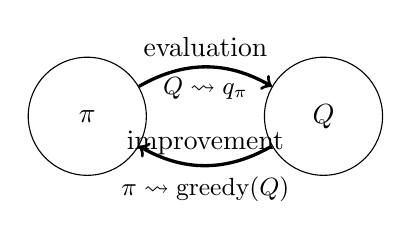
\begin{tikzpicture}[scale=1.5]
    % Nodes
    \node[draw, circle, minimum size=1.5cm] (pi) at (0,1) {$\pi$};
    \node[draw, circle, minimum size=1.5cm] (Q) at (2,1) {$Q$};
    
    % Arrows
    \draw[->, very thick] (pi) to[bend left=30] node[above] {evaluation} node[below] {\small $Q \rightsquigarrow q_\pi$} (Q);
    \draw[->, very thick] (Q) to[bend left=30] node[above] {improvement} node[below] {\small $\pi \rightsquigarrow \text{greedy}(Q)$} (pi);
\end{tikzpicture}
\end{center}

\vspace{1em}
\textbf{반복 과정:}
\begin{enumerate}
    \item \textbf{Policy Evaluation:} 현재 policy $\pi$에 대해 $Q^\pi(s,a)$ 추정
    \item \textbf{Policy Improvement:} $Q$에 대해 greedy하게 policy 개선
\end{enumerate}
\end{frame}

\begin{frame}{MC Control Algorithm}
\textbf{1. Policy Improvement:} 현재 value function에 대해 greedy하게 policy 개선
\[
\pi(s) = \arg\max_{a \in \mathcal{A}} Q(s, a)
\]

\vspace{0.5em}
\textbf{2. Generate Episode:} 새 policy $\pi$로 새 episode 생성
\begin{itemize}
    \item $\varepsilon$-greedy 같은 알고리즘 사용하여 exploration과 exploitation 균형
\end{itemize}

\vspace{0.5em}
\textbf{3. Estimate $Q$:} 새 episode로 $Q$ 추정
\[
q_\pi(s, a) = \frac{\sum_{t=1}^{T} \left( 1[S_t=s, A_t=a] \sum_{k=0}^{T-t-1} \gamma^k R_{t+k+1} \right)}{\sum_{t=1}^{T} 1[S_t=s, A_t=a]}
\]

\vspace{0.5em}
이 과정을 수렴할 때까지 반복
\end{frame}

\begin{frame}{$\varepsilon$-Greedy Exploration}
\textbf{문제:} 순수 greedy policy는 exploration이 부족할 수 있음

\vspace{1em}
\textbf{$\varepsilon$-Greedy Solution:}
\begin{itemize}
    \item 확률 $1-\varepsilon$로: 현재 최선의 action 선택 (exploitation)
    \[
    a = \arg\max_{a'} Q(s, a')
    \]
    \item 확률 $\varepsilon$로: 랜덤하게 action 선택 (exploration)
    \[
    a \sim \text{Uniform}(\mathcal{A})
    \]
\end{itemize}

\vspace{1em}
\textbf{Trade-off:}
\begin{itemize}
    \item $\varepsilon$가 크면: 더 많은 exploration, 느린 수렴
    \item $\varepsilon$가 작으면: 더 많은 exploitation, local optimum 위험
\end{itemize}
\end{frame}

\begin{frame}{MC의 한계 (1): 높은 Variance}
\textbf{문제:} Return의 variance가 크면 sample이 많이 필요함

\vspace{1em}
\textbf{이유:}
\begin{itemize}
    \item Return $G = R_1 + \gamma R_2 + \gamma^2 R_3 + \cdots$
    \item 미래에 일어나는 여러 random 요소가 쌓임
    \item $\Rightarrow$ Variance가 커지기 쉬움
\end{itemize}

\vspace{1em}
\textbf{결과:}
\begin{itemize}
    \item 평균이 안정되려면 sample을 많이 모아야 함
    \item 추정 품질이 천천히 좋아짐
    \item Data efficiency가 낮음
\end{itemize}
\end{frame}

\begin{frame}{MC의 한계 (2): Reset 불가}
\textbf{문제:} State를 특정 위치로 "reset"하는 게 어려운 경우가 많음

\vspace{1em}
MC는 "state $s$에서 시작하는 독립 실험"이 필요한데...

\vspace{0.5em}
현실에서는:
\begin{itemize}
    \item 특정 state로 돌아가는 게 \textbf{불가능}
    \begin{itemize}
        \item 예: 공항 운영, 전력망, 금융 시장
    \end{itemize}
    \item Reset 비용이 너무 \textbf{비쌈}
    \item \textbf{Online/실시간}으로 계속 돌아가야 함
    \begin{itemize}
        \item "$s$로 돌아가서 다시 해볼게요"가 안 됨
    \end{itemize}
\end{itemize}

\vspace{0.5em}
$\Rightarrow$ 억지로 MC 쓰면 \textbf{bias}가 생길 수 있음
\end{frame}

\begin{frame}{대안: TD (Temporal Difference) Learning}
\textbf{핵심 아이디어:}

\vspace{0.5em}
\begin{center}
\large{Episode 끝날 때까지 기다리지 말고,} \\
\large{한 step 보고 바로 update하자!}
\end{center}

\vspace{1em}
\textbf{TD(0) Update Rule:}
\[
V(S_t) \leftarrow V(S_t) + \alpha \Big( \underbrace{R_{t+1} + \gamma V(S_{t+1})}_{\text{TD target}} - V(S_t) \Big)
\]

\vspace{0.5em}
\textbf{TD Error:}
\[
\delta_t = R_{t+1} + \gamma V(S_{t+1}) - V(S_t)
\]

\vspace{0.3em}
\small{Bellman equation을 써서 다음 state의 estimate로 \textbf{bootstrapping}}

\small{TD는 \textbf{Markov property 활용}: 현재 state $S_t$와 다음 state $S_{t+1}$만으로 update}
\end{frame}

\begin{frame}{MC vs TD: Target 비교}
\textbf{MC Target:} 실제 Return (episode 끝까지 기다림)
\[
G_t = R_{t+1} + \gamma R_{t+2} + \gamma^2 R_{t+3} + \cdots
\]

\vspace{1em}
\textbf{TD Target:} Bootstrapped estimate (한 step만 기다림)
\[
R_{t+1} + \gamma V(S_{t+1})
\]

\vspace{1em}
\begin{center}
\begin{tabular}{c|c|c}
 & \textbf{MC} & \textbf{TD} \\
\hline
Target & 실제 $G_t$ & $R_{t+1} + \gamma V(S_{t+1})$ \\
기다리는 시간 & Episode 끝 & 한 step \\
Bias & 없음 & 있음 (bootstrapping) \\
Variance & 높음 & 낮음 \\
\end{tabular}
\end{center}
\end{frame}

\begin{frame}{MC vs TD: 시각적 비교}
\begin{center}
\includegraphics[width=1\textwidth]{images/mc-td.png}
\end{center}
\end{frame}

\begin{frame}{Bias-Variance Trade-off}
\begin{center}
\begin{tabular}{c|c|c}
 & \textbf{Bias} & \textbf{Variance} \\
\hline
MC & Low & High \\
TD & High & Low \\
\end{tabular}
\end{center}

\vspace{0.5em}
\textbf{MC:}
\begin{itemize}
    \item 실제 return을 쓰므로 unbiased
    \item 하지만 return에 많은 random 요소가 쌓여서 $\rightarrow$ high variance
\end{itemize}

\vspace{0.5em}
\textbf{TD:}
\begin{itemize}
    \item 현재 estimate $V(S_{t+1})$을 쓰므로 biased
    \item 하지만 한 step의 randomness만 관여해서 $\rightarrow$ low variance
\end{itemize}

\vspace{0.3em}
\small{$\gamma$가 작거나 episode가 길수록 TD의 이점이 커짐}
\end{frame}

\begin{frame}{When are Monte Carlo methods preferred over TD?}
\footnotesize
\textbf{Question from Stack Exchange\footnotemark:}

\vspace{0.3em}
``TD-learning uses bootstrapping to approximate the action-value function and Monte Carlo uses an average to accomplish this. I just can't really think of a scenario when MC is the better way to go.''

\vspace{0.5em}
\textbf{Main answer:}

\vspace{0.2em}
TD learning과 DP의 주요 문제는 step updates가 \textbf{초기 조건에 biased}되어 있다는 점. Bootstrapping 과정에서 $Q(s',a')$를 사용하는데, 학습 초기에는 실제 보상 정보를 포함하지 않음.

\vspace{0.3em}
Bias는 점진적으로 감소하지만, 특히 \textbf{off-policy methods}(e.g. Q-Learning)와 \textbf{function approximators}를 함께 사용할 때 문제 발생 $\rightarrow$ \textbf{deadly triad}

\vspace{0.3em}
\textbf{Monte Carlo methods:} 실제 sample을 사용하므로 unbiased. 하지만 \textbf{high variance} $\rightarrow$ 더 많은 samples 필요

\vspace{0.3em}
\textbf{실용적 관점:} TD learning이 더 효율적으로 학습 (deadly triad를 극복할 수 있다면). Experience replay와 frozen estimators가 해결책 (e.g., DQN)

\vspace{0.3em}
\textbf{MC의 실용적 장점:} 개념적으로 단순하고 robust하며 구현이 쉬움. \textbf{Policy evaluation}에 적합 (unbiased measure로 여러 agent 비교 시)

\vspace{0.5em}
\footnotetext[1]{\tiny \url{https://stats.stackexchange.com/questions/336974}}
\end{frame}

\begin{frame}{Tabular TD(0) (1/5): 알고리즘}
\textbf{목표:} 유한한 MRP $M$의 value function $V$를 추정하기

\vspace{0.5em}
$((X_t, R_{t+1}); t \geq 0)$: MRP에서 실제로 관측한 데이터

$\hat{V}_t(x)$: 시간 $t$에서 상태 $x$의 value 추정값 (처음엔 $\hat{V}_0 \equiv 0$)

\vspace{0.5em}
\textbf{TD(0) 업데이트:}
\[
\delta_{t+1} = R_{t+1} + \gamma \hat{V}_t(X_{t+1}) - \hat{V}_t(X_t)
\]
\[
\hat{V}_{t+1}(x) = \hat{V}_t(x) + \alpha_t \delta_{t+1} \mathbb{I}\{X_t = x\}, \quad x \in \mathcal{X}
\]

\vspace{0.5em}
\textbf{핵심:}
\begin{itemize}
    \item 방금 방문한 상태 $X_t$의 값만 업데이트함
    \item $\alpha_t \leq 1$이면: 현재 값을 목표값 $R_{t+1} + \gamma \hat{V}_t(X_{t+1})$ 쪽으로 조금씩 이동
    \item \textbf{TD error} $\delta_{t+1}$: 연속된 두 시점의 상태 가치 차이
\end{itemize}
\end{frame}

\begin{frame}{TD(0)}
\begin{center}
\includegraphics[width=0.85\textwidth]{images/td0.png}
\end{center}

\vspace{0.3em}
\small{TD(0)는 한 step만 보고 바로 업데이트 (bootstrapping)}
\end{frame}

\begin{frame}[fragile]{Tabular TD(0) (2/5): 의사코드}
\begin{lstlisting}[language=Python, caption=TD(0) Implementation]
def TD0(X, R, Y, V, alpha, gamma):
    """
    X: last state
    R: immediate reward
    Y: next state
    V: array storing current value estimates
    """
    delta = R + gamma * V[Y] - V[X]
    V[X] = V[X] + alpha * delta
    return V
\end{lstlisting}

\vspace{0.5em}
\textbf{특징:}
\begin{itemize}
    \item 매 transition마다 호출됨
    \item Bootstrapping 사용: 다음 상태의 추정값 $\hat{V}(X_{t+1})$를 활용
    \item Stochastic Approximation (확률적 근사) 알고리즘
\end{itemize}
\end{frame}

\begin{frame}{Tabular TD(0) (3/5): 수렴성}
\textbf{수렴 원리:} TD(0)가 수렴하면 $\hat{V}$는 다음을 만족:
\[
F_{\hat{V}}(x) = \mathbb{E}[R_{t+1} + \gamma \hat{V}(X_{t+1}) - \hat{V}(X_t) \mid X_t = x] = 0
\]

\vspace{0.5em}
간단히 계산하면: $F_{\hat{V}} = T\hat{V} - \hat{V}$ ($T$는 Bellman operator)

\vspace{0.5em}
$F_{\hat{V}} = 0$의 유일한 해는 참 value function $V$ $\Rightarrow$ TD(0)는 $V$로 수렴

\vspace{1em}
\textbf{수렴 조건:} $(X_t; t \in \mathbb{N})$이 stationary, ergodic Markov chain이고, step-size가 Robbins-Monro 조건을 만족하면:
\[
\sum_{t=0}^{\infty} \alpha_t = \infty, \quad \sum_{t=0}^{\infty} \alpha_t^2 < +\infty
\]

$\hat{V}_t$는 거의 확실히 $V$로 수렴
\end{frame}

\begin{frame}{Tabular TD(0) (4/5): Step-Size 설정하기}
\textbf{이론적으로 좋은 step-size (Robbins-Monro 조건):}
\begin{itemize}
    \item $\alpha_t = c/t$ (가장 단순한 형태)
    \item 일반적으로: $\alpha_t = ct^{-\eta}$, 단 $1/2 < \eta \leq 1$
    \begin{itemize}
        \item $\eta = 1$: 장기적으로 최선 (step-size가 제일 천천히 감소)
        \item $\eta \to 1/2$: 초기 학습이 빠름 (step-size가 천천히 감소)
    \end{itemize}
\end{itemize}

\vspace{0.5em}
\textbf{실전에선 고정 step-size를 많이 씀:}
\begin{itemize}
    \item 이론적 조건은 안 맞지만, 실용적인 이유가 있음:
    \begin{enumerate}
        \item \textbf{환경이 변할 때}: Policy가 계속 바뀌는 경우
        \item \textbf{데이터가 적을 때}: 샘플이 충분하지 않은 경우
    \end{enumerate}
    \item 고정 step-size 쓰면: 분포 수렴 (분산이 step-size에 비례)
\end{itemize}

\vspace{0.5em}
\textbf{수렴 속도:} Linear SA이므로 $O(1/\sqrt{t})$
\end{frame}

\begin{frame}{Tabular TD(0) (5/5): Off-Policy 학습}
\textbf{더 일반적인 형태:} $((X_t, R_{t+1}, Y_{t+1}); t \geq 0)$ 데이터에도 적용 가능

\vspace{0.3em}
$(X_t; t \geq 0)$은 임의의 ergodic Markov chain, $(Y_{t+1}, R_{t+1}) \sim P(\cdot | X_t)$

\vspace{0.5em}
\textbf{TD error만 바꾸면 됨:}
\[
\delta_{t+1} = R_{t+1} + \gamma \hat{V}(Y_{t+1}) - \hat{V}(X_t)
\]

\vspace{0.5em}
\textbf{이렇게 쓸 수 있음:}
\begin{enumerate}
    \item \textbf{시뮬레이터로 상태 제어}: MRP와 무관하게 $\{X_t\}$ 분포를 조절 가능
    \item \textbf{Off-policy 학습}: 한 policy를 따라가면서 다른 policy를 평가
    \begin{itemize}
        \item 여러 policy를 동시에 학습할 수 있음
    \end{itemize}
    \item \textbf{에피소드 문제}: 종료 상태에 도달하면 초기 분포 $P_0$에서 다시 시작
    \begin{itemize}
        \item "재시작이 있는 연속 샘플링"
    \end{itemize}
\end{enumerate}
\end{frame}

\begin{frame}{TD(0) vs MC: 수렴 속도 비교 (1/3)}
\textbf{상황에 따라 다름.} 구체적 예시로 살펴보자.

\vspace{0.5em}
\textbf{예제 MRP (Figure 4):}
\begin{itemize}
    \item 초기 state: state 1 (확률 0.9) 또는 state 2 (확률 0.1)
    \item State 1 $\to$ 0 $\to$ 3 $\to$ 4 (종료)
    \item State 2 $\to$ 3 $\to$ 4 (종료)
    \item State 3 $\to$ 4로 갈 때만 보상: $R \sim \text{Bernoulli}(0.5)$
    \item 나머지 transition은 보상 0
\end{itemize}

\vspace{0.5em}
\textbf{핵심 관찰:}
\begin{itemize}
    \item State 1은 자주 방문 (90\%)
    \item State 2는 가끔 방문 (10\%)
    \item State 3은 state 2보다 약 10배 자주 방문
\end{itemize}
\end{frame}

\begin{frame}{TD(0) vs MC: 수렴 속도 비교 (2/3)}
\small
\textbf{Case 1: TD(0)가 더 빠른 경우}

State 3에서 보상이 Bernoulli(0.5)로 random일 때:

\vspace{0.3em}
\textbf{TD(0)의 장점:}
\begin{itemize}
    \item State 2를 $k$번째 방문 시, state 3은 약 $10k$번 방문
    \item State 3의 estimate 정확: $\text{Var}[\hat{V}_t(3)] \approx 1/(10k)$
    \item State 2는 정확한 estimate를 target으로 사용
    \item 시간에 따라 target 정확도 향상
\end{itemize}

\vspace{0.3em}
\textbf{MC의 한계:}
\begin{itemize}
    \item State 3 estimate 무시, Bernoulli 보상 직접 사용
    \item $\text{Var}[R_t | X_t = 2] = 0.25$ 계속 유지
    \item Target variance 불변 $\Rightarrow$ 수렴 느림
\end{itemize}

\vspace{0.2em}
$\Rightarrow$ \textbf{Bootstrapping이 도움됨!}
\end{frame}

\begin{frame}{TD(0) vs MC: 수렴 속도 비교 (3/3)}
\footnotesize
\textbf{Case 2: MC가 더 빠른 경우}

State 3 $\to$ 4의 보상이 deterministic하게 1일 때:

\textbf{MC의 장점:}
\begin{itemize}
    \item $R_t = 1$이 정확한 target
    \item 바로 정확한 값으로 업데이트, 빠르게 수렴
\end{itemize}

\vspace{0.15em}
\textbf{TD(0)의 한계:}
\begin{itemize}
    \item State 2 값이 정확해지려면 State 3 estimate가 먼저 정확해져야 함
    \item 연쇄 과정으로 수렴 느림
\end{itemize}

\vspace{0.15em}
\textbf{극단적 예:} Chain $1 \to 2 \to \cdots \to N$
\begin{itemize}
    \item MC: $N$과 무관하게 일정
    \item TD(0): $N$ 증가 시 느려짐
\end{itemize}

\vspace{0.15em}
$\Rightarrow$ \textbf{상황에 따라 선택.}
\end{frame}

\begin{frame}{TD($\lambda$): MC와 TD(0)의 통합 (1/5)}
\textbf{핵심 아이디어:} MC와 TD(0)를 통합하는 방법이 존재

\vspace{0.5em}
\textbf{TD($\lambda$) family (Sutton, 1984, 1988):}
\begin{itemize}
    \item $\lambda \in [0, 1]$: MC와 TD(0) 사이를 보간하는 파라미터
    \item $\lambda = 0$: TD(0)
    \item $\lambda = 1$: MC (every-visit)
    \item $0 < \lambda < 1$: 중간 형태 (multi-step method)
\end{itemize}

\vspace{0.5em}
\textbf{Multi-step return:}
\[
R_{t:k} = \sum_{s=t}^{t+k} \gamma^{s-t} R_{s+1} + \gamma^{k+1} \hat{V}_t(X_{t+k+1})
\]

\vspace{0.3em}
\small{$k$-step 동안의 실제 보상 + bootstrapping}

\vspace{0.5em}
TD($\lambda$)는 이러한 multi-step returns를 exponential weights $(1-\lambda)\lambda^k$로 혼합
\end{frame}

\begin{frame}{TD($\lambda$)}
\begin{center}
\includegraphics[width=0.85\textwidth]{images/tdlambda.png}
\end{center}

\vspace{0.3em}
\small{TD($\lambda$)는 $\lambda$ 값에 따라 MC($\lambda=1$)와 TD(0)($\lambda=0$) 사이를 보간}
\end{frame}

\begin{frame}{TD($\lambda$): MC와 TD(0)의 통합 (2/5)}
\textbf{Eligibility Traces:} Incremental 구현의 핵심

\vspace{0.3em}
\textbf{Accumulating traces:}
\begin{align*}
\delta_{t+1} &= R_{t+1} + \gamma \hat{V}_t(X_{t+1}) - \hat{V}_t(X_t) \\
z_{t+1}(x) &= \mathbb{I}\{x = X_t\} + \gamma \lambda z_t(x) \\
\hat{V}_{t+1}(x) &= \hat{V}_t(x) + \alpha_t \delta_{t+1} z_{t+1}(x)
\end{align*}

초기값: $z_0(x) = 0$

\vspace{0.3em}
\textbf{Trace} $z_t(x)$:
\begin{itemize}
    \item TD error가 value 업데이트에 미치는 영향 조절
    \item 최근 방문 state일수록 큰 값
    \item $\gamma\lambda$로 지수적 감쇠
\end{itemize}
\end{frame}

\begin{frame}{TD($\lambda$): MC와 TD(0)의 통합 (3/5)}
\textbf{Replacing traces:}
\[
z_{t+1}(x) = \max(\mathbb{I}\{x = X_t\}, \gamma \lambda z_t(x))
\]

\vspace{0.3em}
\textbf{Accumulating vs Replacing:}
\begin{itemize}
    \item \textbf{Accumulating}: 방문마다 누적
    \item \textbf{Replacing}: 방문 시 1로 리셋
    \item 실전에선 replacing이 더 나은 경우 많음
\end{itemize}

\vspace{0.3em}
\textbf{Parameter $\lambda$:}
\begin{itemize}
    \item Bootstrapping 정도 조절
    \item $\lambda = 0$: TD(0)
    \item $\lambda = 1$: MC
\end{itemize}
\end{frame}

\begin{frame}[fragile]{TD($\lambda$): MC와 TD(0)의 통합 (4/5)}
\textbf{Pseudocode (Replacing traces):}

\begin{lstlisting}[language=Python, caption=TD(lambda) with Replacing Traces]
def TDLambda(X, R, Y, V, z, alpha, gamma, lam):
    """
    z: array storing eligibility traces
    lam: lambda parameter
    """
    delta = R + gamma * V[Y] - V[X]
    
    for x in States:
        z[x] = gamma * lam * z[x]
        if X == x:
            z[x] = 1
        V[x] = V[x] + alpha * delta * z[x]
    
    return V, z
\end{lstlisting}

\vspace{0.3em}
\small{모든 state의 value를 매 step마다 업데이트 (trace에 비례)}
\end{frame}

\begin{frame}{TD($\lambda$): MC와 TD(0)의 통합 (5/5)}
\small
\textbf{극한 경우의 동작:}
\begin{itemize}
    \item $\lambda = 0$: TD(0)와 동일
    \item $\lambda = 1$ + accumulating traces: Every-visit MC와 동일 (episodic)
    \item $\lambda = 1$ + replacing traces: First-visit MC와 동일 (undiscounted)
\end{itemize}

\vspace{0.3em}
\textbf{실전 팁:}
\begin{itemize}
    \item $\lambda$는 trial and error로 결정
    \item 학습 중에 $\lambda$를 변경해도 수렴성 유지
\end{itemize}

\vspace{0.3em}
\textbf{장점:}
\begin{itemize}
    \item MRP의 value function 추정
    \item Non-episodic 문제에 사용 가능
    \item 적절한 $\lambda$로 MC나 TD(0)보다 훨씬 빠른 수렴
\end{itemize}
\end{frame}

\begin{frame}{Large State Space 문제 (1/3)}
\textbf{문제:} State space가 크거나 무한할 때 tabular 방식 불가능

\vspace{0.3em}
\textbf{해결책: Function Approximation}
\[
V_\theta(x) = \theta^\top \phi(x), \quad x \in \mathcal{X}
\]

\begin{itemize}
    \item $\theta \in \mathbb{R}^d$: Parameter vector
    \item $\phi: \mathcal{X} \to \mathbb{R}^d$: Feature extraction
    \item $\phi_i(x)$: State $x$의 features
\end{itemize}

\vspace{0.3em}
\textbf{핵심:}
\begin{itemize}
    \item 모든 state 값 개별 저장 $\rightarrow$ 불가능
    \item Parameter $\theta$로 근사 $\rightarrow$ 가능!
    \item Feature $\phi(x)$가 중요 정보 압축
\end{itemize}
\end{frame}

\begin{frame}{Large State Space 문제 (2/3)}
\small
\textbf{Feature Extraction 방법들:}

\vspace{0.2em}
\textbf{1. Polynomial/Fourier/Wavelet Basis}
\begin{itemize}
    \item 예: $\phi(x) = (1, x, x^2, \ldots, x^{d-1})^\top$
\end{itemize}

\vspace{0.2em}
\textbf{2. Radial Basis Functions (RBF)}
\begin{itemize}
    \item $\phi_i(x) = \exp(-\eta \|x - x^{(i)}\|^2)$, Grid에 Gaussian 배치
\end{itemize}

\vspace{0.2em}
\textbf{3. State Aggregation}
\begin{itemize}
    \item $\phi(x) \in \{0, 1\}^d$, Binary features
    \item 계산 효율적: $V_\theta(x) = \sum_{i: \phi_i(x)=1} \theta_i$
\end{itemize}

\vspace{0.2em}
\textbf{4. Tile Coding (CMAC)}
\begin{itemize}
    \item Multiple shifted tilings, $s$-sparse features
\end{itemize}
\end{frame}

\begin{frame}{Large State Space 문제 (3/3)}
\small
\textbf{Curse of Dimensionality:}
\begin{itemize}
    \item $D$-차원을 $\epsilon$ 간격으로 discretize: $d = \epsilon^{-D}$
    \item 예: $\epsilon = 1/2$, $D = 100$ $\Rightarrow$ $d \approx 10^{30}$
\end{itemize}

\vspace{0.2em}
\textbf{왜 때로는 가능한가?}
\begin{itemize}
    \item Intrinsic complexity는 낮을 수 있음
    \item 많은 variable이 irrelevant
    \item State가 low-dim submanifold에 존재
\end{itemize}

\end{frame}

\begin{frame}{TD($\lambda$) with Function Approximation (1/5)}
\textbf{문제:} Large state space에서 TD($\lambda$) 사용하기

\vspace{0.3em}
Parametric function approximation $(V_\theta; \theta \in \mathbb{R}^d)$ 사용:
\begin{itemize}
    \item $V_\theta : \mathcal{X} \to \mathbb{R}$, smooth ($\nabla_\theta V_\theta(x)$ exists)
\end{itemize}

\vspace{0.3em}
\textbf{Tabular TD($\lambda$)의 일반화 (Sutton, 1984, 1988):}
\begin{align*}
\delta_{t+1} &= R_{t+1} + \gamma V_{\theta_t}(X_{t+1}) - V_{\theta_t}(X_t) \\
z_{t+1} &= \nabla_\theta V_{\theta_t}(X_t) + \gamma \lambda z_t \\
\theta_{t+1} &= \theta_t + \alpha_t \delta_{t+1} z_{t+1}
\end{align*}

초기값: $z_0 = 0 \in \mathbb{R}^d$

\vspace{0.3em}
\textbf{핵심 차이:}
\begin{itemize}
    \item Tabular: $z_t(x)$ (각 state마다)
    \item Function approx: $z_t \in \mathbb{R}^d$ (parameter space)
\end{itemize}
\end{frame}

\begin{frame}{TD($\lambda$) with Function Approximation}
\begin{center}
\includegraphics[width=1\textwidth]{images/tdlambda-fa.png}
\end{center}

\vspace{0.3em}
\small{TD($\lambda$)를 function approximation과 결합하여 large state space에서 사용}
\end{frame}

\begin{frame}[fragile]{TD($\lambda$) with Function Approximation (2/5)}
\small
\textbf{Linear Function Approximation:} $V_\theta(x) = \theta^\top \phi(x)$

\vspace{0.2em}
$\nabla_\theta V_\theta = \phi$이므로 업데이트가 단순해짐:

\begin{lstlisting}[language=Python, caption=TD(lambda) with Linear Function Approx]
def TDLambdaLinFA(X, R, Y, theta, z, phi, alpha, gamma, lam):
    """
    phi: feature function
    """
    delta = R + gamma * theta.dot(phi(Y)) - theta.dot(phi(X))
    z = phi(X) + gamma * lam * z
    theta = theta + alpha * delta * z
    return theta, z
\end{lstlisting}

\vspace{0.2em}
\textbf{Tabular case 복원:}
\begin{itemize}
    \item $\mathcal{X} = \{x_1, \ldots, x_D\}$, $\phi_i(x) = \mathbb{I}\{x = x_i\}$
    \item $z_{t,i} \leftrightarrow z_t(x_i)$, $\theta_{t,i} \leftrightarrow \hat{V}_t(x_i)$
\end{itemize}
\end{frame}

\begin{frame}{TD($\lambda$) with Function Approximation (3/5)}
\small
\textbf{수렴 조건 (Linear case):}

TD($\lambda$)가 거의 확실하게 수렴하려면:
\begin{enumerate}
    \item Linear function approximation: $V_\theta = \theta^\top \phi$
    \item $(X_t; t \geq 0)$이 ergodic Markov process
    \item Stationary distribution $\mu$가 MRP와 동일
    \item Step-size가 RM 조건 만족
\end{enumerate}

\vspace{0.2em}
\textbf{수렴 시 만족하는 식:} Projected fixed-point equation
\[
V_{\theta^{(\lambda)}} = \Pi_{F,\mu} T^{(\lambda)} V_{\theta^{(\lambda)}}
\]

\begin{itemize}
    \item $F = \{V_\theta | \theta \in \mathbb{R}^d\}$: Representable functions
    \item $T^{(\lambda)}$: Exponentially weighted Bellman operator
    \item $\Pi_{F,\mu}$: Projection onto $F$ w.r.t. $\|\cdot\|_\mu$
\end{itemize}

\vspace{0.2em}
\textbf{주의:} Off-policy나 nonlinear function approx 시 발산 가능!
\end{frame}

\begin{frame}{TD($\lambda$) with Function Approximation (4/5)}
\small
\textbf{Multi-step Bellman Operator:}
\[
T^{[m]} \hat{V}(x) = \mathbb{E}\left[ \sum_{t=0}^{m} \gamma^t R_{t+1} + \gamma^{m+1} \hat{V}(X_{m+1}) \,\Big|\, X_0 = x \right]
\]

\textbf{TD($\lambda$) Operator:}
\[
T^{(\lambda)} \hat{V}(x) = (1-\lambda) \sum_{m=0}^{\infty} \lambda^m T^{[m]} \hat{V}(x)
\]

특수한 경우: $\lambda = 0 \Rightarrow T^{(0)} = T$, $\lambda = 1 \Rightarrow T^{(1)} = V$

\vspace{0.2em}
\textbf{Error Bound:}
\[
\|V_{\theta^{(\lambda)}} - V\|_\mu \leq \frac{1}{\sqrt{1 - \gamma_\lambda}} \|\Pi_{F,\mu} V - V\|_\mu
\]

여기서 $\gamma_\lambda = \gamma(1-\lambda)/(1-\lambda\gamma)$ (contraction modulus)

\vspace{0.2em}
\begin{itemize}
    \item $\lambda = 1$: Best approximation in $F$
    \item $\lambda \to 0$: Bound가 커짐 (더 큰 error 허용)
\end{itemize}
\end{frame}

\begin{frame}{TD($\lambda$) with Function Approximation (5/5)}
\small
\textbf{TD($\lambda$)가 해결하는 Model:}

Bellman error: $\Delta^{(\lambda)}(\hat{V}) = T^{(\lambda)} \hat{V} - \hat{V}$

\vspace{0.2em}
Error decomposition:
\[
\Delta^{(\lambda)}(V_{\theta^{(\lambda)}}) = (1-\lambda) \sum_{m \geq 0} \lambda^m \Delta_m^{[r]} + \gamma \left( (1-\lambda) \sum_{m \geq 0} \lambda^m \Delta_m^{[\phi]} \right) \theta^{(\lambda)}
\]

\begin{itemize}
    \item $\Delta_m^{[r]}$: $m$-step reward modeling error
    \item $\Delta_m^{[\phi]}$: $m$-step transition modeling error
\end{itemize}

\vspace{0.2em}
\textbf{해석:}
\begin{itemize}
    \item $\lambda \to 1$: Features가 value function 구조를 잘 잡아야 함
    \item $\lambda \to 0$: Features가 immediate rewards/transitions를 잘 잡아야 함
    \item Best $\lambda$는 features가 short-term vs long-term 중 어느 것을 더 잘 capture하는지에 따라 달라짐
\end{itemize}

\vspace{0.2em}
\textbf{실전:} TD($\lambda$) with $\lambda < 1$이 TD(1)보다 훨씬 빠르게 수렴
\end{frame}

\begin{frame}{Gradient Temporal Difference Learning (1/4)}
\textbf{문제:} TD($\lambda$)의 off-policy divergence

\vspace{0.3em}
TD($\lambda$)는 off-policy 상황에서 발산 가능 $\Rightarrow$ 안정성 문제

\vspace{0.3em}
\textbf{해결책:} GTD2 \& TDC (Sutton et al., 2009)
\begin{itemize}
    \item Off-policy에서도 수렴 보장
    \item On-policy에서 TD($\lambda$) 솔루션으로 수렴
    \item TD($\lambda$)와 거의 같은 계산 효율성
\end{itemize}

\vspace{0.3em}
\textbf{설정:} $\lambda = 0$ (TD(0)), linear function approximation
\begin{itemize}
    \item $(X_t, R_{t+1}, Y_{t+1})$: Stationary process
    \item $X_t \sim \nu$ ($\nu$는 stationary distribution과 다를 수 있음)
    \item Features $\phi$는 linearly independent
\end{itemize}

\vspace{0.3em}
\textbf{핵심 아이디어:} Projected fixed-point equation의 solution $\theta^{(0)}$를 찾되, gradient 기반 방법 사용
\end{frame}

\begin{frame}{Gradient Temporal Difference Learning (2/4)}
\small
\textbf{Objective Function:}
\[
J(\theta) = \|V_\theta - \Pi_{F,\nu} T V_\theta\|_\nu^2
\]

\begin{itemize}
    \item Projected fixed-point equation의 모든 solution은 $J$의 minimizer
    \item Linear independent features $\Rightarrow$ unique minimizer $\theta^*$
\end{itemize}

\vspace{0.2em}
\textbf{Notation:}
\begin{align*}
\delta_{t+1}(\theta) &= R_{t+1} + \gamma V_\theta(Y_{t+1}) - V_\theta(X_t) \\
&= R_{t+1} + \gamma \theta^\top \phi_{t+1}' - \theta^\top \phi_t
\end{align*}

여기서 $\phi_t = \phi(X_t)$, $\phi_{t+1}' = \phi(Y_{t+1})$

\vspace{0.2em}
\textbf{Gradient:}
\[
\nabla_\theta J(\theta) = -2 \mathbb{E}[(\phi_t - \gamma \phi_{t+1}') \phi_t^\top] w(\theta)
\]

여기서 $w(\theta) = \mathbb{E}[\phi_t \phi_t^\top]^{-1} \mathbb{E}[\delta_{t+1}(\theta) \phi_t]$
\end{frame}

\begin{frame}[fragile]{Gradient Temporal Difference Learning (3/4)}
\footnotesize
\textbf{GTD2 Algorithm:} Two sets of weights - $\theta_t$ (primary), $w_t$ (auxiliary)

Update rules:
\begin{align*}
\theta_{t+1} &= \theta_t + \alpha_t (\phi_t - \gamma \phi_{t+1}') \phi_t^\top w_t \\
w_{t+1} &= w_t + \beta_t (\delta_{t+1}(\theta_t) - \phi_t^\top w_t) \phi_t
\end{align*}

\begin{lstlisting}[language=Python, caption=GTD2 Implementation]
def GTD2(X, R, Y, theta, w, phi, alpha, beta, gamma):
    f = phi(X)
    f_prime = phi(Y)
    delta = R + gamma * theta.dot(f_prime) - theta.dot(f)
    a = f.dot(w)
    theta = theta + alpha * (f - gamma * f_prime) * a
    w = w + beta * (delta - a) * f
    return theta, w
\end{lstlisting}

\textbf{특징:} $w_t$ 업데이트는 LMS (Least-Mean Square) rule 사용
\end{frame}

\begin{frame}{GTD2: Visualization}
\begin{center}
\includegraphics[width=1\textwidth]{images/gtd2.png}
\end{center}
\end{frame}

\begin{frame}{Gradient Temporal Difference Learning (5/5)}
\small
\textbf{TDC (TD with Corrections):}

Alternative gradient formulation:
\begin{align*}
\theta_{t+1} &= \theta_t + \alpha_t (\delta_{t+1}(\theta_t) \phi_t - \gamma \phi_{t+1}' \phi_t^\top w_t) \\
w_{t+1} &= w_t + \beta_t (\delta_{t+1}(\theta_t) - \phi_t^\top w_t) \phi_t
\end{align*}

\textbf{주요 차이:}
\begin{itemize}
    \item GTD2: $\theta$ update에서 $(\phi_t - \gamma \phi_{t+1}') \phi_t^\top w_t$
    \item TDC: $\theta$ update에서 $\delta_{t+1} \phi_t - \gamma \phi_{t+1}' \phi_t^\top w_t$
    \item TDC는 two-timescale SA: $\alpha_t = o(\beta_t)$ 필요
\end{itemize}

\vspace{0.2em}
\textbf{수렴 보장:}
\begin{itemize}
    \item RM 조건 하에서 $\theta_t \to \theta^*$ almost surely
    \item Distribution $\nu$와 무관하게 수렴 (off-policy 안전!)
    \item Computational cost: TD(0)의 약 2배
\end{itemize}

\vspace{0.2em}
\textbf{확장:} Eligibility traces, nonlinear function approximation으로 확장 가능
\end{frame}

\begin{frame}{Least-Squares Methods (1/9)}
\textbf{기존 방법들의 한계:}

TD($\lambda$), GTD2, TDC는 모두 LMS 스타일의 작은 스텝 업데이트
\begin{itemize}
    \item Step-size 선택에 민감
    \item 초기값과 limit point $\theta^{(\lambda)}$의 거리에 민감
    \item Matrix $A$의 eigenvalue 구조에 영향 받음 \\
    (예: TD(0)의 경우 $A = \mathbb{E}[\phi_t(\phi_t - \gamma\phi'_{t+1})^\top]$)
\end{itemize}

\vspace{0.3em}
\textbf{개선 시도들:}
\begin{itemize}
    \item Adaptive step-sizes (Sutton, 1992)
    \item Normalizing updates (Bradtke, 1994)
    \item Reusing previous samples (Lin, 1992)
    \item 각각 장단점 존재
\end{itemize}

\vspace{0.3em}
\textbf{해결책:} Adaptive filtering의 LS (Least-Squares) 알고리즘을 RL에 적용 \\
$\Rightarrow$ LMS의 모든 결점 해결
\end{frame}

\begin{frame}{LSTD: Least-Squares TD Learning (2/9)}
\small
\textbf{핵심 아이디어:}

TD(0)는 무한 샘플의 극한에서 다음을 만족하는 $\theta$ 찾음:
\[
\mathbb{E}[\phi_t \delta_{t+1}(\theta)] = 0
\]

\vspace{0.2em}
유한 샘플 $D_n = ((X_0, R_1, Y_1), \ldots, (X_{n-1}, R_n, Y_n))$로 근사:
\[
\frac{1}{n} \sum_{t=0}^{n-1} \phi_t \delta_{t+1}(\theta) = 0
\]

\vspace{0.2em}
$\delta_{t+1}(\theta) = R_{t+1} - (\phi_t - \gamma\phi'_{t+1})^\top\theta$를 대입하면 $\theta$에 대한 선형 방정식!

\vspace{0.2em}
$\hat{A}_n = \frac{1}{n}\sum_{t=0}^{n-1} \phi_t(\phi_t - \gamma\phi'_{t+1})^\top$가 non-singular이면:
\[
\theta_n = \hat{A}_n^{-1} \hat{b}_n
\]

여기서 $\hat{b}_n = \frac{1}{n}\sum_{t=0}^{n-1} R_{t+1}\phi_t$
\end{frame}

\begin{frame}{LSTD: Least-Squares TD Learning (3/9)}
\textbf{LSTD의 장점:}
\begin{itemize}
    \item TD(0)보다 빠른 수렴 (eigenvalue spread에 영향 받지 않음)
    \item Sample average approximation 사용
    \item Projected squared Bellman error의 empirical approximation 최소화: \\
    $\|\Pi_{F,\mu}(TV - V)\|_\mu^2$
\end{itemize}

\vspace{0.3em}
\textbf{LSTD의 단점:}
\begin{itemize}
    \item Matrix inversion 필요 ($d$가 크면 비용 증가)
    \item 자주 호출되면 계산 부담
\end{itemize}

\vspace{0.3em}
\textbf{제안:} Bradtke \& Barto (1996)

\vspace{0.3em}
\textbf{통계적 관점:}
\begin{itemize}
    \item Stochastic programming: Sample average approximation
    \item Statistics: Z-estimation family
\end{itemize}
\end{frame}

\begin{frame}[fragile]{RLSTD: Recursive LSTD (4/9)}
\small
\textbf{Sherman-Morrison formula 활용:} Incremental version of LSTD

\vspace{0.2em}
초기화: $\theta_0 \in \mathbb{R}^d$, $C_0 = \beta I$ ($\beta > 0$ small)

\vspace{0.2em}
업데이트 ($t \geq 0$):
\begin{align*}
C_{t+1} &= C_t - \frac{C_t \phi_t(\phi_t - \gamma\phi'_{t+1})^\top C_t}{1 + (\phi_t - \gamma\phi'_{t+1})^\top C_t \phi_t} \\
\theta_{t+1} &= \theta_t + \frac{C_t}{1 + (\phi_t - \gamma\phi'_{t+1})^\top C_t \phi_t} \delta_{t+1}(\theta_t) \phi_t
\end{align*}

\vspace{0.2em}
\textbf{계산 복잡도:} $O(d^2)$ per update

\vspace{0.2em}
\textbf{특징:}
\begin{itemize}
    \item Adaptive filtering의 RLS (Recursive Least-Squares)와 유사
    \item Online learning에 적합
    \item Matrix inversion을 incremental하게 수행
\end{itemize}
\end{frame}

\begin{frame}{RLSTD: Visualization}
\begin{center}
\includegraphics[width=1\textwidth]{images/rlstd.png}
\end{center}
\end{frame}

\begin{frame}{LSTD($\lambda$): Extension to Eligibility Traces (5/9)}
\small
\textbf{LSTD($\lambda$)} (Boyan, 2002): $\lambda$ parameter 추가

\vspace{0.2em}
\textbf{전제조건:} $\lambda > 0$일 때 $X_{t+1} = Y_{t+1}$ 필요 (TD errors가 telescope하려면)

\vspace{0.2em}
Solution은 다음을 만족:
\[
\frac{1}{n} \sum_{t=0}^{n-1} \delta_{t+1}(\theta) z_{t+1} = 0
\]

여기서 $z_{t+1} = \sum_{s=0}^{t} (\gamma\lambda)^{t-s} \phi_s$ (eligibility traces)

\vspace{0.2em}
\textbf{Recursive form:} RLSTD($\lambda$) (Xu et al., 2002; Nedić \& Bertsekas, 2003)

\vspace{0.2em}
\textbf{문제점:} Equation (30)이 해를 갖지 않을 수 있음
\begin{itemize}
    \item On-policy + 큰 샘플: 항상 해 존재
    \item 해가 없을 때의 trick: Small positive diagonal matrix 추가 \\
    (보장 안됨)
    \item \textbf{Better approach:} Projected Bellman error 최소화 \\
    (항상 well-defined)
\end{itemize}
\end{frame}

\begin{frame}{LSTD($\lambda$): Convergence Properties (6/9)}
\textbf{수렴성:}

Standard assumptions 하에서 LSTD($\lambda$) (및 recursive variants)는 projected fixed-point equation (22)의 solution으로 almost surely 수렴

\vspace{0.3em}
\textbf{이론적 결과:}
\begin{itemize}
    \item $\lambda = 0$: Bradtke \& Barto (1996)
    \item $\lambda > 0$: Xu et al. (2002), Nedić \& Bertsekas (2003)
    \item On-policy case에서 증명되었으나, off-policy에서도 성립 \\
    (limiting solution이 존재한다면)
\end{itemize}

\vspace{0.3em}
\textbf{(R)LSTD($\lambda$)의 장점:}
\begin{itemize}
    \item Step-size 튜닝 불필요
    \item Matrix $A$의 eigenvalue 구조에 민감하지 않음
    \item 초기값 $\theta$의 선택에 민감하지 않음
\end{itemize}

\vspace{0.3em}
\textbf{실험적 확인:} TD($\lambda$)보다 빠른 수렴 (Bradtke \& Barto, 1996; Boyan, 2002; Xu et al., 2002)
\end{frame}

\begin{frame}[fragile]{LSPE: Least-Squares Policy Evaluation (7/9)}
\small
\textbf{$\lambda$-LSPE} (Bertsekas \& Ioffe, 1996): Multi-step value iteration 모방

\vspace{0.2em}
$(n-s)$-step prediction:
\[
\hat{V}^{(\lambda)}_{s,n}(\theta) = \theta^\top\phi_s + \sum_{q=s}^{n-1} (\gamma\lambda)^{q-s} \delta_{q+1}(\theta)
\]

Loss function:
\[
J_n(\hat{\theta}, \theta) = \frac{1}{n} \sum_{s=0}^{n-1} \left( \hat{\theta}^\top\phi_s - \hat{V}^{(\lambda)}_{s,n}(\theta) \right)^2
\]

Update:
\[
\theta_{t+1} = \theta_t + \alpha_t \left( \arg\min_{\hat{\theta}} J_{n_t}(\hat{\theta}, \theta_t) - \theta_t \right)
\]

여기서 $(n_t; t \geq 0)$는 non-decreasing integer sequence

\vspace{0.2em}
\textbf{특징:} $J_n$은 $\hat{\theta}$에 대해 quadratic $\Rightarrow$ closed form solution
\end{frame}

\begin{frame}{$\lambda$-LSPE: Visualization}
\begin{center}
\includegraphics[width=1\textwidth]{images/lambdalspe.png}
\end{center}
\end{frame}

\begin{frame}{LSPE: Properties and Comparison (9/9)}
\small
\textbf{특별 케이스} ($\lambda = 0$, $\alpha_t = 1$):
\[
\theta_{t+1} = \arg\min_{\hat{\theta}} \frac{1}{n_t} \sum_{s=0}^{n_t-1} \{\hat{\theta}^\top\phi(X_s) - (R_{s+1} + \gamma V_{\theta_t}(Y_{s+1}))\}^2
\]
$\Rightarrow$ Fitted value iteration with linear function approximation

\vspace{0.2em}
\textbf{$\alpha_t < 1$의 역할:}
\begin{itemize}
    \item 작은 샘플에서 parameter 안정화
    \item Control algorithm의 subroutine으로 사용 시 policy를 점진적으로 변경
\end{itemize}

\vspace{0.2em}
\textbf{수렴성:} Standard assumptions + $n_t = t$ 하에서 almost surely 수렴
\begin{itemize}
    \item Decreasing step-sizes (Nedić \& Bertsekas, 2003)
    \item Constant step-sizes: $0 < \alpha < \frac{2-2\gamma\lambda}{1+\gamma-2\gamma\lambda}$ (항상 1 포함)
\end{itemize}
\end{frame}

\begin{frame}{Least-Squares vs TD-like Methods (1/3)}
\small
\textbf{계산 복잡도 비교 (샘플 크기 $n$):}

\vspace{0.2em}
\begin{tabular}{lll}
\textbf{Method} & \textbf{Complexity} & \textbf{비고} \\
\hline
LSTD & $O(nd^2 + d^3)$ & Matrix inversion \\
RLSTD & $O(nd^2)$ & Recursive update \\
LSPE & $O(nd^2)$ & \\
TD($\lambda$) & $O(nd)$ & Lightweight \\
GTD2/TDC & $O(nd)$ & Lightweight \\
\end{tabular}

\vspace{0.2em}
\textbf{Trade-off:}
\begin{itemize}
    \item Least-squares: 높은 안정성 \& 정확도 $\Leftrightarrow$ 높은 계산 복잡도
    \item Lightweight: 낮은 복잡도 $\Leftrightarrow$ step-size 민감
\end{itemize}

\vspace{0.2em}
\textbf{Observation:} Lightweight는 least-squares가 1번 pass하는 동안 $d$번 pass 가능!

\vspace{0.2em}
\textbf{Experience Replay} (Lin, 1992): 관측을 저장/재사용하여 정확도 향상
\end{frame}

\begin{frame}{Least-Squares vs TD-like Methods (2/3)}
\small
\textbf{$d$가 매우 큰 경우:}

\begin{itemize}
    \item Lightweight methods가 같은 계산 시간 내에 least-squares만큼 성능 발휘 가능
    \item 예: Go 게임의 value function (Silver et al., 2007) - 백만 개 이상의 features 사용
    \item 이 경우 least-squares methods는 실행 불가능
\end{itemize}

\vspace{0.3em}
\textbf{분석 시나리오:} 새로운 관측이 negligible cost로 가능한 경우
\begin{itemize}
    \item 데이터 저장/재사용 불필요
    \item 성능은 계산 속도에 의존
\end{itemize}

\vspace{0.3em}
\textbf{계산 시간 $T$ 고정 시:}
\begin{itemize}
    \item Least-squares: 샘플 크기 $n \approx T/d^2$ 처리 가능
    \item Lightweight methods: 샘플 크기 $n' \approx nd = T/d$ 처리 가능
\end{itemize}

\vspace{0.3em}
$\Rightarrow$ Lightweight methods가 $d$배 많은 샘플 처리!
\end{frame}

\begin{frame}{Least-Squares vs TD-like Methods (3/3)}
\footnotesize
\textbf{정확도 비교:} Limit parameter $\theta^*$

수렴 속도:
\begin{align*}
\|\theta_t - \theta^*\| &\approx C_1 t^{-1/2} \quad \text{(LSTD)} \\
\|\theta'_t - \theta^*\| &\approx C_2 t^{-1/2} \quad \text{(TD-like)}
\end{align*}

같은 계산 시간 $T$ 후의 정확도 비율:
\[
\frac{\|\theta'_{n'} - \theta^*\|}{\|\theta_n - \theta^*\|} \approx \frac{C_2}{C_1} d^{-1/2}
\]

\vspace{0.1em}
\textbf{결론:}
\begin{itemize}
    \item $C_2/C_1 < d^{1/2}$: Lightweight TD-like 방법이 더 정확
    \item $C_2/C_1 > d^{1/2}$: Least-squares 방법이 더 정확
    \item \textbf{경험적 rule:} $d$ 작으면 least-squares, $d$ 크면 lightweight
\end{itemize}

\vspace{0.1em}
\textbf{iLSTD} (Geramifard et al., 2007): Incremental LSTD
\begin{itemize}
    \item Sparse features ($s$ nonzero): Complexity $O(sd)$ per iteration
    \item Storage: $O(\min(ns^2 + d, d^2))$
    \item $ns^2 \ll d^2$일 때 경쟁적
\end{itemize}
\end{frame}

\begin{frame}{Function Space 선택 (1/8)}
\textbf{Value function 품질 측정:}

목표가 value-prediction일 때, 적절한 state distribution $\mu$에 대한 MSE (Mean-Squared Error) 사용

\vspace{0.3em}
\textbf{Learning의 관점:}

Function space $F$에서 함수 선택: $F = \{V_\theta \mid \theta \in \mathbb{R}^d\}$

\vspace{0.3em}
\textbf{Approximation Error:}
\[
\inf_{V_\theta \in F} \|V_\theta - V^*\|_\mu
\]

\begin{itemize}
    \item 더 큰 function space $\Rightarrow$ 작은 approximation error
    \item 예: Linear approximation에서 독립적인 features 추가
\end{itemize}

\vspace{0.3em}
\textbf{문제:} Incomplete information을 사용하는 learning에서 function space 크기 증가는 양날의 검!
\begin{itemize}
    \item Approximation error $\downarrow$, but Estimation error $\uparrow$
\end{itemize}
\end{frame}

\begin{frame}{Function Space 선택 (2/8)}
\textbf{단순화된 분석:}

Linear approximation + LSTD, $\gamma = 0$, $(X_t, R_{t+1})$ i.i.d., $X_t \sim \mu$

\vspace{0.3em}
이 경우: $V(x) = r(x) = \mathbb{E}[R_{t+1}|X_t = x]$

\vspace{0.3em}
LSTD는 empirical loss의 minimizer 계산:
\[
L_n(\theta) = \frac{1}{n} \sum_{t=0}^{n-1} (\theta^\top \phi(X_t) - R_{t+1})^2
\]

\vspace{0.3em}
\textbf{핵심 질문:}
\begin{itemize}
    \item Feature dimensionality $d$가 클 때 어떤 일이 발생하는가?
    \item Sample size $n$과 $d$의 관계는?
\end{itemize}
\end{frame}

\begin{frame}{Function Space 선택 (3/8)}
\textbf{Overfitting 시나리오:}

$d \geq n$이고 feature matrix가 full row rank라면:

\vspace{0.3em}
\begin{itemize}
    \item $L_n$의 minimum = 0
    \item LSTD solution $\theta_n$: $\theta_n^\top \phi(X_t) = R_{t+1}$ for all $t$
    \item Perfect fit on training data!
\end{itemize}

\vspace{0.3em}
\textbf{문제점:}
\begin{itemize}
    \item Noisy rewards $\Rightarrow$ 큰 estimation error
    \item $\|\theta_n^\top \phi - V\|_\mu$ 매우 큼
    \item \textbf{Overfitting:} Model이 "noise"에 fitting됨
\end{itemize}

\vspace{0.3em}
\textbf{해결책:} 더 작은 $d$ (더 작은 $F$) 선택
\begin{itemize}
    \item Overfitting 감소
    \item But: Approximation error 증가
    \item $\Rightarrow$ Tradeoff 존재!
\end{itemize}
\end{frame}

\begin{frame}{Function Space 선택 (4/8)}
\textbf{Tradeoff 정량화:}

$\theta^*$: True loss의 minimizer
\[
\theta^* = \arg\min_\theta L(\theta), \quad L(\theta) = \mathbb{E}[(\theta^\top \phi(X_t) - R_{t+1})^2]
\]

\vspace{0.3em}
$V_{\theta^*}$는 $V$의 $F$로의 projection

\vspace{0.3em}
\textbf{핵심 아이디어:}
\begin{itemize}
    \item LSTD는 $\theta^*$를 근사
    \item 하지만 유한 샘플 $\Rightarrow$ Estimation error 발생
    \item Function space 크기에 따라 error가 달라짐
\end{itemize}
\end{frame}

\begin{frame}{Function Space 선택 (5/8)}
\small
\textbf{통계적 bound} (Györfi et al., 2002):

Bounded rewards ($|R| \leq R$) + truncation 가정:
\[
\mathbb{E}[\|\theta_n^\top \phi - V\|_\mu^2] \leq C_1 \frac{d(1 + \log n)}{n} + C_2 \|(\theta^*)^\top \phi - V\|_\mu^2
\]

\vspace{0.3em}
\textbf{항목 분석:}
\begin{itemize}
    \item \textbf{첫 번째 항:} Estimation error bound
    \begin{itemize}
        \item $d$ 증가 $\Rightarrow$ 증가
        \item $n$ 증가 $\Rightarrow$ 감소
    \end{itemize}
    \item \textbf{두 번째 항:} Approximation error
    \begin{itemize}
        \item $d$ 증가 $\Rightarrow$ (일반적으로) 감소
    \end{itemize}
\end{itemize}

\vspace{0.3em}
\textbf{Constants:}
\begin{itemize}
    \item $C_1$: Reward의 variance \& range에 비례
    \item $C_2$: Universal constant
\end{itemize}
\end{frame}

\begin{frame}{Function Space 선택 (6/8)}
\begin{center}
\includegraphics[width=0.85\textwidth]{images/convergence-figure-5.png}
\end{center}

\vspace{0.2em}
\small
\textbf{핵심 아이디어:}
\begin{itemize}
    \item $L_n(\theta) \to L(\theta)$ for any fixed $\theta$ (Law of large numbers)
    \item 하지만 $L_n(\cdot)$가 $L(\cdot)$에 uniformly close하지 않을 수 있음
    \item $\Rightarrow$ $L_n$의 minimizer가 작은 true loss $L$을 주지 않을 수 있음
    \item Uniform closeness 보장이 $d$가 클수록 어려움
\end{itemize}
\end{frame}

\begin{frame}{Function Space 선택 (7/8)}
\footnotesize
\textbf{일반화:}

Similar bounds는 다음 경우에도 성립:
\begin{itemize}
    \item $\gamma > 0$
    \item Dependent sequence $(X_t; t \geq 0)$ (잘 mixing하면)
    \item $\gamma \neq 0$: Noise는 $R_{t+1}$과 $Y_{t+1}$ 모두에서 발생
\end{itemize}

\textbf{Control algorithms에서도:}
\begin{itemize}
    \item Fitted value iteration (Munos \& Szepesvári, 2008)
    \item Fitted actor-critic (Antos et al., 2007)
    \item Approximate policy iteration (Antos et al., 2008)
    \item Finite-sample performance bounds 존재
\end{itemize}

\textbf{결론:} Approximation-Estimation tradeoff는 RL의 근본적인 문제
\begin{itemize}
    \item Function space 너무 크면: Overfitting (high variance)
    \item Function space 너무 작으면: Underfitting (high bias)
\end{itemize}
\end{frame}

\begin{frame}{Function Space 선택 (8/9)}
\small
\textbf{자동 Feature Selection \& Regularization:}

Function space 선택의 중요성과 어려움 인식 $\Rightarrow$ 자동화 연구 증가

\vspace{0.2em}
\textbf{Parsimonious basis functions 구성:}
\begin{itemize}
    \item Gaussian RBF 파라미터 튜닝 (Menache et al., 2005)
    \item Nonparametric techniques (Keller et al., 2006; Parr et al., 2007)
    \item Numerical analysis + nonparametric (Mahadevan, 2009)
\end{itemize}

\vspace{0.2em}
\textbf{Supervised learning 기법 활용:}
\begin{itemize}
    \item Regression trees (Ernst et al., 2005)
    \item Kernel methods (Rasmussen \& Kuss, 2004; Engel et al., 2005)
    \item $\ell_1$-regularization (LASSO-inspired, Kolter \& Ng, 2009)
    \item Regularization with statistical guarantees (Farahmand et al., 2009)
\end{itemize}
\end{frame}

\begin{frame}{Function Space 선택 (9/9)}
\textbf{개사기 Neural Network의 등장:}

\vspace{0.3em}
\textbf{개레전드 Neural Networks가 제공하는 것:}
\begin{itemize}
    \item \textbf{Universal Approximation:} 충분한 크기의 네트워크는 임의의 연속 함수 근사 가능
    \item \textbf{Automatic Feature Learning:} Hand-crafted features 대신 데이터로부터 representation 학습
    \item \textbf{Scalability:} 고차원 state/action spaces 처리 가능
    \item \textbf{End-to-End Learning:} Raw sensory input부터 action까지 직접 학습
\end{itemize}

\vspace{0.3em}
\textbf{마침내. Deep Reinforcement Learning의 시작:}
\begin{itemize}
    \item DQN (Mnih et al., 2015): Atari 게임을 raw pixels로부터 학습
    \item 이전 방법들과 달리 feature engineering 불필요
    \item TD learning + Deep Neural Networks의 결합
    \item Experience replay \& Target networks로 안정성 확보
\end{itemize}

\vspace{0.3em}
\textbf{현대 RL의 방향:} Function approximation의 선택이 linear에서 deep neural networks로 확장
\end{frame}

% ============================================
\section{Control}
% ============================================

% ============================================
\section{For Further Exploration}
% ============================================

% ============================================
% References
% ============================================

\begin{frame}[allowframebreaks]{참고문헌}
    \textbf{주요 참고 자료:}
    
    \vspace{0.8em}
    \begin{enumerate}
        \item \textbf{Szepesvári, C. (2009).} \\
        \textit{Algorithms for Reinforcement Learning} \\
        Synthesis Lectures on Artificial Intelligence and Machine Learning, \\
        Morgan \& Claypool Publishers \\
        \small{\url{https://sites.ualberta.ca/~szepesva/rlbook.html}}
        
        \vspace{0.5em}
        \item \textbf{Sutton, R. S., \& Barto, A. G. (2018).} \\
        \textit{Reinforcement Learning: An Introduction (2nd ed.)} \\
        MIT Press
        
        \vspace{0.5em}
        \item \textbf{Kaelbling, L. P., Littman, M. L., \& Moore, A. W. (1996).} \\
        \textit{Reinforcement Learning: A Survey} \\
        Journal of Artificial Intelligence Research (JAIR), 4, 237-285
        
        \vspace{0.5em}
        \item \textbf{Silver, D.} \\
        \textit{UCL Course on Reinforcement Learning - Lecture 1: Introduction to RL}
        
        \vspace{0.5em}
        \item \textbf{Zhou, Y. (2019).} \\
        \textit{IE 498: Online Learning and Decision Making} \\
        Fall 2019, University of Illinois at Urbana-Champaign \\
        Teaching Assistant: Tanmay Gangwani
        
        \vspace{0.5em}
        \item \textbf{Bertsekas, D. P. (2019).} \\
        \textit{Reinforcement Learning and Optimal Control} \\
        Athena Scientific
        
        \vspace{0.5em}
        \item \textbf{Ng, A.} \\
        \textit{CS229 Lecture Notes - Reinforcement Learning and Control} \\
        Stanford University
        
        \vspace{0.5em}
        \item \textbf{Dayan, P., \& Niv, Y. (2008).} \\
        \textit{Reinforcement learning: The Good, The Bad and The Ugly} \\
        Current Opinion in Neurobiology, 18(2), 185-196
        
        \vspace{0.5em}
        \item \textbf{Mnih, V., et al. (2015).} \\
        \textit{Human-level control through deep reinforcement learning} \\
        Nature, 518(7540), 529-533
        
        \vspace{0.5em}
        \item \textbf{Pineau, J.} \\
        \textit{Beyond Bellman's Legacy: Rethinking What we Value}
        
        \vspace{0.5em}
        \item \textbf{Weng, L. (2018).} \\
        \textit{A (Long) Peek into Reinforcement Learning} \\
        Lil'Log Blog \\
        \small{\url{https://lilianweng.github.io/posts/2018-02-19-rl-overview/}}
        
        \vspace{0.5em}
        \item \textbf{Stack Exchange Discussion (2018).} \\
        \textit{When are Monte Carlo methods preferred over temporal difference ones?} \\
        Cross Validated \\
        \small{\url{https://stats.stackexchange.com/questions/336974}}
    \end{enumerate}
    
    \vspace{0.5em}
    \small{\textit{본 발표 자료는 위 교재와 논문들을 바탕으로 작성되었습니다.}}
\end{frame}

\end{document}
